% Chapter 3: Simulation tables (and figures)
For each batch of simulations defined by outcome and predictor variable type, the following tables report power, median bias, and coverage probability.

Tables are included in this section 'Simulation', and results are described and summarized in the subsequent section entitled 'Results'.
Tables of results are displayed by trial size ($n$), marginal outcome prevalence ($Pr( Y )$) when the outcome is binary, prognostic factor prevalence ($Pr( X )$) when prognostic factors are binary, treatment effect size ($bZ$), and prognostic factor effect size ($bX$).

Results are reported separately by model adjustment for prognostic factors, 
the treatment allocation method used (CR - complete randomization, SBR - stratified block randomization, CAA: covariate adaptive allocation\footnote{see Section 2.2: \textit{Allocation procedures} for method parameters and implementation details}), 
and analysis type (model-based or rerandomization).

For the batches where binary outcomes are considered, power is reported averaging over the subset of simulation results where the \texttt{glm} algorithm converged and at least one event was observed in each treatment arm.

\newpage

\section[Binary Y, binary X]{Batch 1: Binary Outcome, Binary Predictors}

% Tables \ref{tab:b1p}, \ref{tab:b1mb}, and \ref{tab:b1c} report power, median bias, and coverage probability, respectively. 

\begingroup\fontsize{7}{9}\selectfont
\rowcolors{2}{white}{gray!6}

\begin{longtable}[t]{cccccrrrrrrc}
\caption{\label{tab:b1p}Batch 1 (Binary Y, Binary X): Power}\\
\hiderowcolors
\toprule
\multicolumn{5}{c}{ } & \multicolumn{6}{c}{Model-based} & \multicolumn{1}{c}{Rerandomization} \\
\cmidrule(l{2pt}r{2pt}){6-11} \cmidrule(l{2pt}r{2pt}){12-12}
\multicolumn{5}{c}{ } & \multicolumn{2}{c}{CR} & \multicolumn{2}{c}{SBR} & \multicolumn{2}{c}{CAA} & \multicolumn{1}{c}{CAA} \\
\cmidrule(l{2pt}r{2pt}){6-7} \cmidrule(l{2pt}r{2pt}){8-9} \cmidrule(l{2pt}r{2pt}){10-11} \cmidrule(l{2pt}r{2pt}){12-12}
n & Pr( Y ) & Pr( X ) & bZ & bX & adj & unadj & adj & unadj & adj & unadj & adj\\
\midrule
\showrowcolors
32 & 0.1 & 0.25 & 1.0 & 1.1 & 0.009 & 0.001 & 0.006 & 0.000 & 0.007 & 0.000 & 0.075\\
32 & 0.1 & 0.25 & 1.0 & 3.0 & 0.015 & 0.001 & 0.017 & 0.000 & 0.018 & 0.001 & 0.071\\
32 & 0.1 & 0.25 & 1.1 & 1.1 & 0.009 & 0.001 & 0.007 & 0.000 & 0.008 & 0.000 & 0.077\\
32 & 0.1 & 0.25 & 1.1 & 3.0 & 0.016 & 0.001 & 0.017 & 0.000 & 0.020 & 0.001 & 0.070\\
32 & 0.1 & 0.25 & 3.0 & 1.1 & 0.015 & 0.004 & 0.012 & 0.003 & 0.013 & 0.003 & 0.147\\
32 & 0.1 & 0.25 & 3.0 & 3.0 & 0.024 & 0.007 & 0.025 & 0.004 & 0.026 & 0.007 & 0.157\\
\addlinespace
32 & 0.1 & 0.50 & 1.0 & 1.1 & 0.009 & 0.000 & 0.008 & 0.000 & 0.005 & 0.000 & 0.078\\
32 & 0.1 & 0.50 & 1.0 & 3.0 & 0.018 & 0.001 & 0.022 & 0.001 & 0.020 & 0.001 & 0.070\\
32 & 0.1 & 0.50 & 1.1 & 1.1 & 0.009 & 0.001 & 0.007 & 0.000 & 0.004 & 0.000 & 0.079\\
32 & 0.1 & 0.50 & 1.1 & 3.0 & 0.019 & 0.002 & 0.021 & 0.000 & 0.022 & 0.001 & 0.071\\
32 & 0.1 & 0.50 & 3.0 & 1.1 & 0.015 & 0.004 & 0.009 & 0.002 & 0.013 & 0.004 & 0.149\\
32 & 0.1 & 0.50 & 3.0 & 3.0 & 0.042 & 0.007 & 0.040 & 0.003 & 0.045 & 0.006 & 0.165\\
\addlinespace
32 & 0.5 & 0.25 & 1.0 & 1.1 & 0.028 & 0.029 & 0.031 & 0.026 & 0.028 & 0.025 & 0.057\\
32 & 0.5 & 0.25 & 1.0 & 3.0 & 0.019 & 0.023 & 0.022 & 0.017 & 0.025 & 0.022 & 0.056\\
32 & 0.5 & 0.25 & 1.1 & 1.1 & 0.025 & 0.027 & 0.027 & 0.022 & 0.033 & 0.029 & 0.063\\
32 & 0.5 & 0.25 & 1.1 & 3.0 & 0.023 & 0.025 & 0.024 & 0.017 & 0.026 & 0.022 & 0.059\\
32 & 0.5 & 0.25 & 3.0 & 1.1 & 0.210 & 0.230 & 0.232 & 0.230 & 0.222 & 0.219 & 0.326\\
32 & 0.5 & 0.25 & 3.0 & 3.0 & 0.172 & 0.192 & 0.197 & 0.181 & 0.198 & 0.182 & 0.302\\
\addlinespace
32 & 0.5 & 0.50 & 1.0 & 1.1 & 0.026 & 0.029 & 0.026 & 0.025 & 0.026 & 0.025 & 0.062\\
32 & 0.5 & 0.50 & 1.0 & 3.0 & 0.022 & 0.025 & 0.028 & 0.016 & 0.024 & 0.019 & 0.059\\
32 & 0.5 & 0.50 & 1.1 & 1.1 & 0.029 & 0.030 & 0.024 & 0.023 & 0.024 & 0.023 & 0.064\\
32 & 0.5 & 0.50 & 1.1 & 3.0 & 0.027 & 0.031 & 0.028 & 0.018 & 0.028 & 0.022 & 0.061\\
32 & 0.5 & 0.50 & 3.0 & 1.1 & 0.202 & 0.226 & 0.223 & 0.223 & 0.223 & 0.228 & 0.327\\
32 & 0.5 & 0.50 & 3.0 & 3.0 & 0.161 & 0.177 & 0.190 & 0.164 & 0.180 & 0.170 & 0.300\\
\addlinespace
96 & 0.1 & 0.25 & 1.0 & 1.1 & 0.026 & 0.018 & 0.024 & 0.019 & 0.026 & 0.018 & 0.058\\
96 & 0.1 & 0.25 & 1.0 & 3.0 & 0.038 & 0.026 & 0.041 & 0.026 & 0.036 & 0.019 & 0.051\\
96 & 0.1 & 0.25 & 1.1 & 1.1 & 0.025 & 0.019 & 0.027 & 0.020 & 0.028 & 0.018 & 0.063\\
96 & 0.1 & 0.25 & 1.1 & 3.0 & 0.038 & 0.027 & 0.040 & 0.025 & 0.039 & 0.022 & 0.055\\
96 & 0.1 & 0.25 & 3.0 & 1.1 & 0.226 & 0.210 & 0.213 & 0.205 & 0.224 & 0.207 & 0.358\\
96 & 0.1 & 0.25 & 3.0 & 3.0 & 0.270 & 0.245 & 0.274 & 0.241 & 0.278 & 0.242 & 0.376\\
\addlinespace
96 & 0.1 & 0.50 & 1.0 & 1.1 & 0.024 & 0.018 & 0.025 & 0.017 & 0.026 & 0.018 & 0.060\\
96 & 0.1 & 0.50 & 1.0 & 3.0 & 0.045 & 0.024 & 0.044 & 0.021 & 0.048 & 0.026 & 0.061\\
96 & 0.1 & 0.50 & 1.1 & 1.1 & 0.025 & 0.019 & 0.023 & 0.018 & 0.027 & 0.019 & 0.061\\
96 & 0.1 & 0.50 & 1.1 & 3.0 & 0.047 & 0.026 & 0.045 & 0.021 & 0.049 & 0.025 & 0.060\\
96 & 0.1 & 0.50 & 3.0 & 1.1 & 0.217 & 0.212 & 0.219 & 0.207 & 0.232 & 0.218 & 0.363\\
96 & 0.1 & 0.50 & 3.0 & 3.0 & 0.308 & 0.267 & 0.328 & 0.277 & 0.318 & 0.267 & 0.394\\
\addlinespace
96 & 0.5 & 0.25 & 1.0 & 1.1 & 0.043 & 0.045 & 0.044 & 0.048 & 0.038 & 0.045 & 0.050\\
96 & 0.5 & 0.25 & 1.0 & 3.0 & 0.046 & 0.047 & 0.045 & 0.041 & 0.043 & 0.041 & 0.055\\
96 & 0.5 & 0.25 & 1.1 & 1.1 & 0.046 & 0.049 & 0.049 & 0.052 & 0.046 & 0.052 & 0.057\\
96 & 0.5 & 0.25 & 1.1 & 3.0 & 0.050 & 0.051 & 0.051 & 0.048 & 0.048 & 0.047 & 0.060\\
96 & 0.5 & 0.25 & 3.0 & 1.1 & 0.725 & 0.744 & 0.730 & 0.745 & 0.741 & 0.764 & 0.752\\
96 & 0.5 & 0.25 & 3.0 & 3.0 & 0.680 & 0.649 & 0.691 & 0.675 & 0.683 & 0.672 & 0.704\\
\addlinespace
96 & 0.5 & 0.50 & 1.0 & 1.1 & 0.044 & 0.047 & 0.045 & 0.050 & 0.048 & 0.053 & 0.059\\
96 & 0.5 & 0.50 & 1.0 & 3.0 & 0.042 & 0.048 & 0.042 & 0.036 & 0.046 & 0.044 & 0.058\\
96 & 0.5 & 0.50 & 1.1 & 1.1 & 0.045 & 0.047 & 0.049 & 0.054 & 0.050 & 0.056 & 0.059\\
96 & 0.5 & 0.50 & 1.1 & 3.0 & 0.046 & 0.048 & 0.047 & 0.042 & 0.046 & 0.040 & 0.057\\
96 & 0.5 & 0.50 & 3.0 & 1.1 & 0.725 & 0.741 & 0.740 & 0.757 & 0.739 & 0.758 & 0.752\\
96 & 0.5 & 0.50 & 3.0 & 3.0 & 0.661 & 0.629 & 0.676 & 0.647 & 0.669 & 0.648 & 0.694\\
\bottomrule
\end{longtable}
\rowcolors{2}{white}{white}\endgroup{}
 \newpage 
\begingroup\fontsize{7}{9}\selectfont
\rowcolors{2}{white}{gray!6}

\begin{longtable}[t]{cccccrrrrrrc}
\caption{\label{tab:b1mb}Batch 1 (Binary Y, Binary X): Median bias}\\
\hiderowcolors
\toprule
\multicolumn{5}{c}{ } & \multicolumn{6}{c}{Model-based} & \multicolumn{1}{c}{Rerandomization} \\
\cmidrule(l{2pt}r{2pt}){6-11} \cmidrule(l{2pt}r{2pt}){12-12}
\multicolumn{5}{c}{ } & \multicolumn{2}{c}{CR} & \multicolumn{2}{c}{SBR} & \multicolumn{2}{c}{CAA} & \multicolumn{1}{c}{CAA} \\
\cmidrule(l{2pt}r{2pt}){6-7} \cmidrule(l{2pt}r{2pt}){8-9} \cmidrule(l{2pt}r{2pt}){10-11} \cmidrule(l{2pt}r{2pt}){12-12}
n & Pr( Y ) & Pr( X ) & bZ & bX & adj & unadj & adj & unadj & adj & unadj & adj\\
\midrule
\showrowcolors
32 & 0.1 & 0.25 & 1.0 & 1.1 & 0.000 & 0.000 & 0.000 & 0.000 & 0.000 & 0.000 & 0.000\\
32 & 0.1 & 0.25 & 1.0 & 3.0 & 0.000 & 0.000 & 0.000 & 0.000 & 0.000 & 0.000 & 0.000\\
32 & 0.1 & 0.25 & 1.1 & 1.1 & -0.019 & -0.044 & -0.095 & -0.095 & -0.065 & -0.095 & -0.065\\
32 & 0.1 & 0.25 & 1.1 & 3.0 & -0.007 & 0.038 & -0.045 & -0.095 & -0.028 & -0.095 & -0.028\\
32 & 0.1 & 0.25 & 3.0 & 1.1 & 0.297 & 0.167 & 0.196 & 0.143 & 0.237 & 0.143 & 0.237\\
32 & 0.1 & 0.25 & 3.0 & 3.0 & 0.316 & 0.065 & 0.227 & 0.000 & 0.282 & 0.000 & 0.282\\
\addlinespace
32 & 0.1 & 0.50 & 1.0 & 1.1 & 0.000 & 0.000 & 0.000 & 0.000 & 0.000 & 0.000 & 0.000\\
32 & 0.1 & 0.50 & 1.0 & 3.0 & 0.000 & 0.000 & 0.000 & 0.000 & 0.000 & 0.000 & 0.000\\
32 & 0.1 & 0.50 & 1.1 & 1.1 & -0.013 & -0.065 & -0.095 & -0.095 & -0.079 & -0.095 & -0.079\\
32 & 0.1 & 0.50 & 1.1 & 3.0 & 0.028 & 0.022 & -0.011 & -0.095 & -0.031 & -0.095 & -0.031\\
32 & 0.1 & 0.50 & 3.0 & 1.1 & 0.289 & 0.143 & 0.173 & 0.065 & 0.284 & 0.143 & 0.284\\
32 & 0.1 & 0.50 & 3.0 & 3.0 & 0.283 & 0.065 & 0.222 & 0.059 & 0.229 & 0.059 & 0.229\\
\addlinespace
32 & 0.5 & 0.25 & 1.0 & 1.1 & 0.012 & 0.000 & 0.000 & 0.000 & 0.000 & 0.000 & 0.000\\
32 & 0.5 & 0.25 & 1.0 & 3.0 & 0.001 & 0.000 & 0.000 & 0.000 & -0.003 & 0.000 & -0.003\\
32 & 0.5 & 0.25 & 1.1 & 1.1 & 0.021 & -0.008 & 0.008 & -0.047 & 0.011 & -0.031 & 0.011\\
32 & 0.5 & 0.25 & 1.1 & 3.0 & 0.030 & -0.026 & 0.009 & -0.047 & -0.006 & -0.047 & -0.006\\
32 & 0.5 & 0.25 & 3.0 & 1.1 & 0.131 & 0.031 & 0.145 & 0.031 & 0.128 & -0.011 & 0.128\\
32 & 0.5 & 0.25 & 3.0 & 3.0 & 0.176 & -0.049 & 0.117 & -0.059 & 0.148 & -0.059 & 0.148\\
\addlinespace
32 & 0.5 & 0.50 & 1.0 & 1.1 & -0.007 & 0.000 & -0.008 & 0.000 & 0.012 & 0.000 & 0.012\\
32 & 0.5 & 0.50 & 1.0 & 3.0 & -0.003 & 0.000 & -0.014 & 0.000 & 0.000 & 0.000 & 0.000\\
32 & 0.5 & 0.50 & 1.1 & 1.1 & -0.002 & -0.031 & -0.014 & -0.047 & 0.012 & -0.047 & 0.012\\
32 & 0.5 & 0.50 & 1.1 & 3.0 & 0.006 & -0.047 & -0.004 & -0.047 & -0.010 & -0.080 & -0.010\\
32 & 0.5 & 0.50 & 3.0 & 1.1 & 0.136 & 0.031 & 0.168 & 0.031 & 0.133 & 0.000 & 0.133\\
32 & 0.5 & 0.50 & 3.0 & 3.0 & 0.144 & -0.087 & 0.153 & -0.077 & 0.149 & -0.077 & 0.149\\
\addlinespace
96 & 0.1 & 0.25 & 1.0 & 1.1 & 0.004 & 0.000 & 0.001 & 0.000 & 0.002 & 0.000 & 0.002\\
96 & 0.1 & 0.25 & 1.0 & 3.0 & 0.001 & 0.000 & -0.002 & 0.000 & -0.005 & 0.000 & -0.005\\
96 & 0.1 & 0.25 & 1.1 & 1.1 & 0.009 & 0.002 & -0.004 & -0.004 & -0.007 & -0.013 & -0.007\\
96 & 0.1 & 0.25 & 1.1 & 3.0 & -0.001 & -0.004 & -0.001 & -0.002 & 0.006 & -0.013 & 0.006\\
96 & 0.1 & 0.25 & 3.0 & 1.1 & 0.081 & 0.047 & 0.084 & 0.047 & 0.077 & 0.047 & 0.077\\
96 & 0.1 & 0.25 & 3.0 & 3.0 & 0.065 & -0.045 & 0.071 & -0.047 & 0.062 & -0.047 & 0.062\\
\addlinespace
96 & 0.1 & 0.50 & 1.0 & 1.1 & 0.007 & 0.000 & 0.005 & 0.000 & 0.000 & 0.000 & 0.000\\
96 & 0.1 & 0.50 & 1.0 & 3.0 & -0.001 & 0.000 & 0.018 & 0.000 & 0.001 & 0.000 & 0.001\\
96 & 0.1 & 0.50 & 1.1 & 1.1 & 0.009 & 0.000 & 0.002 & -0.002 & -0.009 & -0.035 & -0.009\\
96 & 0.1 & 0.50 & 1.1 & 3.0 & 0.006 & -0.013 & 0.017 & 0.002 & 0.011 & 0.000 & 0.011\\
96 & 0.1 & 0.50 & 3.0 & 1.1 & 0.085 & 0.054 & 0.070 & 0.047 & 0.093 & 0.054 & 0.093\\
96 & 0.1 & 0.50 & 3.0 & 3.0 & 0.062 & -0.037 & 0.065 & -0.036 & 0.077 & -0.036 & 0.077\\
\addlinespace
96 & 0.5 & 0.25 & 1.0 & 1.1 & 0.013 & 0.007 & 0.002 & 0.000 & 0.001 & 0.000 & 0.001\\
96 & 0.5 & 0.25 & 1.0 & 3.0 & 0.016 & 0.009 & 0.000 & 0.000 & 0.007 & 0.000 & 0.007\\
96 & 0.5 & 0.25 & 1.1 & 1.1 & 0.006 & -0.001 & -0.004 & -0.011 & -0.001 & -0.011 & -0.001\\
96 & 0.5 & 0.25 & 1.1 & 3.0 & 0.021 & 0.007 & -0.002 & -0.012 & 0.015 & -0.010 & 0.015\\
96 & 0.5 & 0.25 & 3.0 & 1.1 & 0.039 & 0.013 & 0.037 & 0.013 & 0.038 & 0.013 & 0.038\\
96 & 0.5 & 0.25 & 3.0 & 3.0 & 0.046 & -0.084 & 0.039 & -0.078 & 0.036 & -0.078 & 0.036\\
\addlinespace
96 & 0.5 & 0.50 & 1.0 & 1.1 & -0.008 & -0.005 & -0.005 & 0.000 & 0.005 & 0.000 & 0.005\\
96 & 0.5 & 0.50 & 1.0 & 3.0 & -0.007 & 0.000 & -0.008 & 0.000 & 0.005 & 0.000 & 0.005\\
96 & 0.5 & 0.50 & 1.1 & 1.1 & -0.002 & -0.008 & -0.001 & -0.009 & 0.001 & -0.008 & 0.001\\
96 & 0.5 & 0.50 & 1.1 & 3.0 & 0.013 & -0.007 & 0.011 & -0.012 & -0.002 & -0.012 & -0.002\\
96 & 0.5 & 0.50 & 3.0 & 1.1 & 0.042 & 0.013 & 0.041 & 0.017 & 0.037 & 0.013 & 0.037\\
96 & 0.5 & 0.50 & 3.0 & 3.0 & 0.037 & -0.112 & 0.032 & -0.143 & 0.041 & -0.136 & 0.041\\
\bottomrule
\end{longtable}
\rowcolors{2}{white}{white}\endgroup{}
 \newpage
\begingroup\fontsize{7}{9}\selectfont
\rowcolors{2}{white}{gray!6}

\begin{longtable}[t]{cccccrrrrrr}
\caption{\label{tab:b1c}Batch 1 (Binary Y, Binary X): Coverage probability}\\
\hiderowcolors
\toprule
\multicolumn{5}{c}{ } & \multicolumn{6}{c}{Model-based} \\
\cmidrule(l{2pt}r{2pt}){6-11}
\multicolumn{5}{c}{ } & \multicolumn{2}{c}{CR} & \multicolumn{2}{c}{SBR} & \multicolumn{2}{c}{CAA} \\
\cmidrule(l{2pt}r{2pt}){6-7} \cmidrule(l{2pt}r{2pt}){8-9} \cmidrule(l{2pt}r{2pt}){10-11}
n & Pr( Y ) & Pr( X ) & bZ & bX & adj & unadj & adj & unadj & adj & unadj\\
\midrule
\showrowcolors
32 & 0.1 & 0.25 & 1.0 & 1.1 & 0.989 & 0.999 & 0.993 & 1.000 & 0.991 & 0.999\\
32 & 0.1 & 0.25 & 1.0 & 3.0 & 0.983 & 0.998 & 0.979 & 0.999 & 0.979 & 0.999\\
32 & 0.1 & 0.25 & 1.1 & 1.1 & 0.989 & 0.999 & 0.992 & 1.000 & 0.990 & 0.999\\
32 & 0.1 & 0.25 & 1.1 & 3.0 & 0.982 & 0.998 & 0.979 & 0.999 & 0.978 & 0.999\\
32 & 0.1 & 0.25 & 3.0 & 1.1 & 0.958 & 0.968 & 0.962 & 0.971 & 0.957 & 0.968\\
32 & 0.1 & 0.25 & 3.0 & 3.0 & 0.969 & 0.979 & 0.959 & 0.975 & 0.957 & 0.975\\
\addlinespace
32 & 0.1 & 0.50 & 1.0 & 1.1 & 0.988 & 0.999 & 0.991 & 0.999 & 0.993 & 0.998\\
32 & 0.1 & 0.50 & 1.0 & 3.0 & 0.979 & 0.998 & 0.974 & 0.998 & 0.975 & 0.998\\
32 & 0.1 & 0.50 & 1.1 & 1.1 & 0.988 & 0.999 & 0.992 & 0.999 & 0.992 & 0.999\\
32 & 0.1 & 0.50 & 1.1 & 3.0 & 0.977 & 0.997 & 0.975 & 0.999 & 0.974 & 0.998\\
32 & 0.1 & 0.50 & 3.0 & 1.1 & 0.954 & 0.966 & 0.959 & 0.967 & 0.954 & 0.967\\
32 & 0.1 & 0.50 & 3.0 & 3.0 & 0.956 & 0.977 & 0.960 & 0.977 & 0.958 & 0.976\\
\addlinespace
32 & 0.5 & 0.25 & 1.0 & 1.1 & 0.963 & 0.954 & 0.958 & 0.948 & 0.964 & 0.956\\
32 & 0.5 & 0.25 & 1.0 & 3.0 & 0.973 & 0.960 & 0.967 & 0.959 & 0.965 & 0.957\\
32 & 0.5 & 0.25 & 1.1 & 1.1 & 0.965 & 0.964 & 0.966 & 0.968 & 0.959 & 0.961\\
32 & 0.5 & 0.25 & 1.1 & 3.0 & 0.969 & 0.967 & 0.966 & 0.971 & 0.965 & 0.967\\
32 & 0.5 & 0.25 & 3.0 & 1.1 & 0.967 & 0.962 & 0.966 & 0.961 & 0.967 & 0.962\\
32 & 0.5 & 0.25 & 3.0 & 3.0 & 0.975 & 0.967 & 0.978 & 0.972 & 0.969 & 0.969\\
\addlinespace
32 & 0.5 & 0.50 & 1.0 & 1.1 & 0.964 & 0.955 & 0.964 & 0.954 & 0.963 & 0.953\\
32 & 0.5 & 0.50 & 1.0 & 3.0 & 0.969 & 0.956 & 0.964 & 0.968 & 0.969 & 0.965\\
32 & 0.5 & 0.50 & 1.1 & 1.1 & 0.963 & 0.960 & 0.969 & 0.968 & 0.969 & 0.968\\
32 & 0.5 & 0.50 & 1.1 & 3.0 & 0.967 & 0.960 & 0.966 & 0.975 & 0.962 & 0.968\\
32 & 0.5 & 0.50 & 3.0 & 1.1 & 0.969 & 0.963 & 0.968 & 0.965 & 0.967 & 0.961\\
32 & 0.5 & 0.50 & 3.0 & 3.0 & 0.973 & 0.959 & 0.972 & 0.966 & 0.973 & 0.968\\
\addlinespace
96 & 0.1 & 0.25 & 1.0 & 1.1 & 0.973 & 0.979 & 0.974 & 0.980 & 0.973 & 0.980\\
96 & 0.1 & 0.25 & 1.0 & 3.0 & 0.959 & 0.971 & 0.956 & 0.971 & 0.960 & 0.979\\
96 & 0.1 & 0.25 & 1.1 & 1.1 & 0.974 & 0.978 & 0.974 & 0.979 & 0.971 & 0.980\\
96 & 0.1 & 0.25 & 1.1 & 3.0 & 0.962 & 0.971 & 0.959 & 0.974 & 0.959 & 0.978\\
96 & 0.1 & 0.25 & 3.0 & 1.1 & 0.972 & 0.974 & 0.975 & 0.977 & 0.972 & 0.974\\
96 & 0.1 & 0.25 & 3.0 & 3.0 & 0.963 & 0.966 & 0.968 & 0.972 & 0.962 & 0.969\\
\addlinespace
96 & 0.1 & 0.50 & 1.0 & 1.1 & 0.974 & 0.980 & 0.974 & 0.981 & 0.971 & 0.980\\
96 & 0.1 & 0.50 & 1.0 & 3.0 & 0.951 & 0.974 & 0.953 & 0.977 & 0.950 & 0.972\\
96 & 0.1 & 0.50 & 1.1 & 1.1 & 0.972 & 0.978 & 0.974 & 0.980 & 0.972 & 0.977\\
96 & 0.1 & 0.50 & 1.1 & 3.0 & 0.950 & 0.972 & 0.955 & 0.977 & 0.949 & 0.973\\
96 & 0.1 & 0.50 & 3.0 & 1.1 & 0.974 & 0.974 & 0.979 & 0.978 & 0.976 & 0.974\\
96 & 0.1 & 0.50 & 3.0 & 3.0 & 0.961 & 0.966 & 0.958 & 0.970 & 0.961 & 0.974\\
\addlinespace
96 & 0.5 & 0.25 & 1.0 & 1.1 & 0.954 & 0.953 & 0.952 & 0.950 & 0.958 & 0.954\\
96 & 0.5 & 0.25 & 1.0 & 3.0 & 0.951 & 0.951 & 0.952 & 0.957 & 0.955 & 0.957\\
96 & 0.5 & 0.25 & 1.1 & 1.1 & 0.957 & 0.956 & 0.954 & 0.952 & 0.956 & 0.952\\
96 & 0.5 & 0.25 & 1.1 & 3.0 & 0.950 & 0.952 & 0.952 & 0.957 & 0.953 & 0.957\\
96 & 0.5 & 0.25 & 3.0 & 1.1 & 0.955 & 0.956 & 0.954 & 0.954 & 0.957 & 0.954\\
96 & 0.5 & 0.25 & 3.0 & 3.0 & 0.952 & 0.944 & 0.952 & 0.952 & 0.957 & 0.951\\
\addlinespace
96 & 0.5 & 0.50 & 1.0 & 1.1 & 0.953 & 0.951 & 0.952 & 0.948 & 0.949 & 0.946\\
96 & 0.5 & 0.50 & 1.0 & 3.0 & 0.955 & 0.950 & 0.956 & 0.963 & 0.951 & 0.956\\
96 & 0.5 & 0.50 & 1.1 & 1.1 & 0.956 & 0.955 & 0.951 & 0.950 & 0.954 & 0.951\\
96 & 0.5 & 0.50 & 1.1 & 3.0 & 0.960 & 0.952 & 0.956 & 0.964 & 0.956 & 0.961\\
96 & 0.5 & 0.50 & 3.0 & 1.1 & 0.952 & 0.953 & 0.953 & 0.953 & 0.952 & 0.954\\
96 & 0.5 & 0.50 & 3.0 & 3.0 & 0.953 & 0.937 & 0.954 & 0.953 & 0.950 & 0.946\\
\bottomrule
\end{longtable}
\rowcolors{2}{white}{white}\endgroup{}
 \newpage

% \begingroup\fontsize{7}{9}\selectfont
\rowcolors{2}{white}{gray!6}

\begin{longtable}[t]{ccccccrrrrrrc}
\caption{\label{tab:b1smb}Batch 1 (Binary Y, Binary X): Median bias, subsetted}\\
\hiderowcolors
\toprule
\multicolumn{6}{c}{ } & \multicolumn{6}{c}{Model-based} & \multicolumn{1}{c}{Rerandomization} \\
\cmidrule(l{2pt}r{2pt}){7-12} \cmidrule(l{2pt}r{2pt}){13-13}
\multicolumn{6}{c}{ } & \multicolumn{2}{c}{CR} & \multicolumn{2}{c}{SBR} & \multicolumn{2}{c}{CAA} & \multicolumn{1}{c}{CAA} \\
\cmidrule(l{2pt}r{2pt}){7-8} \cmidrule(l{2pt}r{2pt}){9-10} \cmidrule(l{2pt}r{2pt}){11-12} \cmidrule(l{2pt}r{2pt}){13-13}
Avg. nsims & n & Pr( Y ) & Pr( X ) & bZ & bX & adj & unadj & adj & unadj & adj & unadj & adj\\
\midrule
\showrowcolors
3452 (68.9\%) & 32 & 0.1 & 0.25 & 1.0 & 1.1 & 0.000 & 0.000 & 0.000 & 0.000 & 0.000 & 0.000 & 0.000\\
3818 (76.2\%) & 32 & 0.1 & 0.25 & 1.0 & 3.0 & 0.000 & 0.000 & 0.000 & 0.000 & 0.000 & 0.000 & 0.000\\
3451 (68.9\%) & 32 & 0.1 & 0.25 & 1.1 & 1.1 & -0.095 & -0.095 & -0.095 & -0.095 & -0.095 & -0.095 & -0.095\\
3804 (75.9\%) & 32 & 0.1 & 0.25 & 1.1 & 3.0 & -0.078 & -0.065 & -0.095 & -0.095 & -0.080 & -0.095 & -0.080\\
3062 (61.1\%) & 32 & 0.1 & 0.25 & 3.0 & 1.1 & -0.389 & -0.435 & -0.403 & -0.470 & -0.402 & -0.405 & -0.402\\
3408 (68\%) & 32 & 0.1 & 0.25 & 3.0 & 3.0 & -0.235 & -0.405 & -0.278 & -0.405 & -0.256 & -0.336 & -0.256\\
\addlinespace
3445 (68.8\%) & 32 & 0.1 & 0.50 & 1.0 & 1.1 & 0.000 & 0.000 & 0.000 & 0.000 & 0.000 & 0.000 & 0.000\\
3868 (77.2\%) & 32 & 0.1 & 0.50 & 1.0 & 3.0 & 0.000 & 0.000 & 0.000 & 0.000 & 0.000 & 0.000 & 0.000\\
3443 (68.7\%) & 32 & 0.1 & 0.50 & 1.1 & 1.1 & -0.087 & -0.095 & -0.095 & -0.095 & -0.095 & -0.095 & -0.095\\
3879 (77.4\%) & 32 & 0.1 & 0.50 & 1.1 & 3.0 & -0.028 & -0.095 & -0.074 & -0.095 & -0.068 & -0.095 & -0.068\\
3053 (60.9\%) & 32 & 0.1 & 0.50 & 3.0 & 1.1 & -0.391 & -0.435 & -0.391 & -0.434 & -0.400 & -0.470 & -0.400\\
3482 (69.5\%) & 32 & 0.1 & 0.50 & 3.0 & 3.0 & -0.223 & -0.351 & -0.218 & -0.336 & -0.234 & -0.336 & -0.234\\
\addlinespace
5008 (100\%) & 32 & 0.5 & 0.25 & 1.0 & 1.1 & 0.012 & 0.000 & 0.000 & 0.000 & 0.000 & 0.000 & 0.000\\
5009 (100\%) & 32 & 0.5 & 0.25 & 1.0 & 3.0 & 0.001 & 0.000 & 0.000 & 0.000 & -0.002 & 0.000 & -0.002\\
5009 (100\%) & 32 & 0.5 & 0.25 & 1.1 & 1.1 & 0.021 & -0.008 & 0.008 & -0.047 & 0.011 & -0.031 & 0.011\\
5009 (100\%) & 32 & 0.5 & 0.25 & 1.1 & 3.0 & 0.030 & -0.026 & 0.009 & -0.047 & -0.006 & -0.047 & -0.006\\
5001 (99.8\%) & 32 & 0.5 & 0.25 & 3.0 & 1.1 & 0.128 & 0.015 & 0.144 & 0.031 & 0.126 & -0.022 & 0.126\\
5001 (99.8\%) & 32 & 0.5 & 0.25 & 3.0 & 3.0 & 0.172 & -0.053 & 0.116 & -0.059 & 0.147 & -0.059 & 0.147\\
\addlinespace
5008 (100\%) & 32 & 0.5 & 0.50 & 1.0 & 1.1 & -0.007 & 0.000 & -0.008 & 0.000 & 0.012 & 0.000 & 0.012\\
5009 (100\%) & 32 & 0.5 & 0.50 & 1.0 & 3.0 & -0.003 & 0.000 & -0.014 & 0.000 & 0.000 & 0.000 & 0.000\\
5009 (100\%) & 32 & 0.5 & 0.50 & 1.1 & 1.1 & -0.003 & -0.031 & -0.014 & -0.047 & 0.012 & -0.047 & 0.012\\
5009 (100\%) & 32 & 0.5 & 0.50 & 1.1 & 3.0 & 0.006 & -0.047 & -0.004 & -0.047 & -0.010 & -0.080 & -0.010\\
5000 (99.8\%) & 32 & 0.5 & 0.50 & 3.0 & 1.1 & 0.133 & 0.031 & 0.167 & 0.031 & 0.132 & 0.000 & 0.132\\
5004 (99.9\%) & 32 & 0.5 & 0.50 & 3.0 & 3.0 & 0.141 & -0.087 & 0.153 & -0.077 & 0.146 & -0.077 & 0.146\\
\addlinespace
4944 (98.7\%) & 96 & 0.1 & 0.25 & 1.0 & 1.1 & 0.003 & 0.000 & 0.000 & 0.000 & 0.000 & 0.000 & 0.000\\
4985 (99.5\%) & 96 & 0.1 & 0.25 & 1.0 & 3.0 & 0.001 & 0.000 & -0.001 & 0.000 & -0.003 & 0.000 & -0.003\\
4939 (98.6\%) & 96 & 0.1 & 0.25 & 1.1 & 1.1 & 0.004 & -0.002 & -0.009 & -0.006 & -0.015 & -0.047 & -0.015\\
4983 (99.5\%) & 96 & 0.1 & 0.25 & 1.1 & 3.0 & -0.001 & -0.004 & -0.002 & -0.003 & 0.006 & -0.013 & 0.006\\
4726 (94.3\%) & 96 & 0.1 & 0.25 & 3.0 & 1.1 & 0.032 & 0.000 & 0.019 & 0.000 & 0.018 & 0.000 & 0.018\\
4877 (97.3\%) & 96 & 0.1 & 0.25 & 3.0 & 3.0 & 0.038 & -0.062 & 0.041 & -0.070 & 0.036 & -0.070 & 0.036\\
\addlinespace
4950 (98.8\%) & 96 & 0.1 & 0.50 & 1.0 & 1.1 & 0.006 & 0.000 & 0.004 & 0.000 & 0.000 & 0.000 & 0.000\\
4992 (99.6\%) & 96 & 0.1 & 0.50 & 1.0 & 3.0 & -0.002 & -0.002 & 0.017 & 0.000 & 0.001 & 0.000 & 0.001\\
4947 (98.7\%) & 96 & 0.1 & 0.50 & 1.1 & 1.1 & 0.007 & -0.003 & -0.001 & -0.002 & -0.013 & -0.047 & -0.013\\
4991 (99.6\%) & 96 & 0.1 & 0.50 & 1.1 & 3.0 & 0.005 & -0.013 & 0.014 & 0.000 & 0.011 & 0.000 & 0.011\\
4752 (94.9\%) & 96 & 0.1 & 0.50 & 3.0 & 1.1 & 0.034 & 0.000 & 0.021 & 0.000 & 0.044 & 0.013 & 0.044\\
4899 (97.8\%) & 96 & 0.1 & 0.50 & 3.0 & 3.0 & 0.044 & -0.050 & 0.049 & -0.047 & 0.060 & -0.045 & 0.060\\
\addlinespace
5010 (100\%) & 96 & 0.5 & 0.25 & 1.0 & 1.1 & 0.013 & 0.007 & 0.002 & 0.000 & 0.001 & 0.000 & 0.001\\
5010 (100\%) & 96 & 0.5 & 0.25 & 1.0 & 3.0 & 0.016 & 0.009 & 0.000 & 0.000 & 0.007 & 0.000 & 0.007\\
5010 (100\%) & 96 & 0.5 & 0.25 & 1.1 & 1.1 & 0.006 & -0.001 & -0.004 & -0.011 & -0.001 & -0.011 & -0.001\\
5010 (100\%) & 96 & 0.5 & 0.25 & 1.1 & 3.0 & 0.021 & 0.007 & -0.002 & -0.012 & 0.015 & -0.010 & 0.015\\
5010 (100\%) & 96 & 0.5 & 0.25 & 3.0 & 1.1 & 0.039 & 0.013 & 0.037 & 0.013 & 0.038 & 0.013 & 0.038\\
5010 (100\%) & 96 & 0.5 & 0.25 & 3.0 & 3.0 & 0.046 & -0.084 & 0.039 & -0.078 & 0.036 & -0.078 & 0.036\\
\addlinespace
5010 (100\%) & 96 & 0.5 & 0.50 & 1.0 & 1.1 & -0.008 & -0.005 & -0.005 & 0.000 & 0.005 & 0.000 & 0.005\\
5010 (100\%) & 96 & 0.5 & 0.50 & 1.0 & 3.0 & -0.007 & 0.000 & -0.008 & 0.000 & 0.005 & 0.000 & 0.005\\
5010 (100\%) & 96 & 0.5 & 0.50 & 1.1 & 1.1 & -0.002 & -0.008 & -0.001 & -0.009 & 0.001 & -0.008 & 0.001\\
5010 (100\%) & 96 & 0.5 & 0.50 & 1.1 & 3.0 & 0.013 & -0.007 & 0.011 & -0.012 & -0.002 & -0.012 & -0.002\\
5010 (100\%) & 96 & 0.5 & 0.50 & 3.0 & 1.1 & 0.042 & 0.013 & 0.041 & 0.017 & 0.037 & 0.013 & 0.037\\
5010 (100\%) & 96 & 0.5 & 0.50 & 3.0 & 3.0 & 0.037 & -0.112 & 0.032 & -0.143 & 0.041 & -0.136 & 0.041\\
\bottomrule
\end{longtable}
\rowcolors{2}{white}{white}\endgroup{}
 \newpage
\begingroup\fontsize{7}{9}\selectfont
\rowcolors{2}{white}{gray!6}

\begin{longtable}[t]{ccccccrrrrrrc}
\caption{\label{tab:b1sp}Batch 1 (Binary Y, Binary X): Power, subsetted}\\
\hiderowcolors
\toprule
\multicolumn{6}{c}{ } & \multicolumn{6}{c}{Model-based} & \multicolumn{1}{c}{Rerandomization} \\
\cmidrule(l{2pt}r{2pt}){7-12} \cmidrule(l{2pt}r{2pt}){13-13}
\multicolumn{6}{c}{ } & \multicolumn{2}{c}{CR} & \multicolumn{2}{c}{SBR} & \multicolumn{2}{c}{CAA} & \multicolumn{1}{c}{CAA} \\
\cmidrule(l{2pt}r{2pt}){7-8} \cmidrule(l{2pt}r{2pt}){9-10} \cmidrule(l{2pt}r{2pt}){11-12} \cmidrule(l{2pt}r{2pt}){13-13}
Avg. nsims & n & Pr( Y ) & Pr( X ) & bZ & bX & adj & unadj & adj & unadj & adj & unadj & adj\\
\midrule
\showrowcolors
3452 (68.9\%) & 32 & 0.1 & 0.25 & 1.0 & 1.1 & 0.006 & 0.001 & 0.003 & 0.000 & 0.003 & 0.001 & 0.017\\
3818 (76.2\%) & 32 & 0.1 & 0.25 & 1.0 & 3.0 & 0.008 & 0.001 & 0.007 & 0.000 & 0.009 & 0.001 & 0.025\\
3451 (68.9\%) & 32 & 0.1 & 0.25 & 1.1 & 1.1 & 0.007 & 0.001 & 0.003 & 0.000 & 0.003 & 0.000 & 0.017\\
3804 (75.9\%) & 32 & 0.1 & 0.25 & 1.1 & 3.0 & 0.008 & 0.001 & 0.008 & 0.001 & 0.010 & 0.001 & 0.024\\
3062 (61.1\%) & 32 & 0.1 & 0.25 & 3.0 & 1.1 & 0.018 & 0.007 & 0.012 & 0.005 & 0.012 & 0.005 & 0.044\\
3408 (68\%) & 32 & 0.1 & 0.25 & 3.0 & 3.0 & 0.024 & 0.010 & 0.022 & 0.006 & 0.025 & 0.010 & 0.065\\
\addlinespace
3445 (68.8\%) & 32 & 0.1 & 0.50 & 1.0 & 1.1 & 0.009 & 0.001 & 0.009 & 0.000 & 0.005 & 0.000 & 0.021\\
3868 (77.2\%) & 32 & 0.1 & 0.50 & 1.0 & 3.0 & 0.021 & 0.002 & 0.025 & 0.001 & 0.022 & 0.001 & 0.022\\
3443 (68.7\%) & 32 & 0.1 & 0.50 & 1.1 & 1.1 & 0.009 & 0.001 & 0.008 & 0.001 & 0.004 & 0.000 & 0.021\\
3879 (77.4\%) & 32 & 0.1 & 0.50 & 1.1 & 3.0 & 0.021 & 0.002 & 0.024 & 0.001 & 0.024 & 0.001 & 0.022\\
3053 (60.9\%) & 32 & 0.1 & 0.50 & 3.0 & 1.1 & 0.019 & 0.007 & 0.013 & 0.003 & 0.018 & 0.006 & 0.046\\
3482 (69.5\%) & 32 & 0.1 & 0.50 & 3.0 & 3.0 & 0.055 & 0.010 & 0.052 & 0.004 & 0.057 & 0.009 & 0.068\\
\addlinespace
5008 (100\%) & 32 & 0.5 & 0.25 & 1.0 & 1.1 & 0.028 & 0.029 & 0.031 & 0.026 & 0.028 & 0.025 & 0.057\\
5009 (100\%) & 32 & 0.5 & 0.25 & 1.0 & 3.0 & 0.019 & 0.023 & 0.022 & 0.017 & 0.025 & 0.022 & 0.056\\
5009 (100\%) & 32 & 0.5 & 0.25 & 1.1 & 1.1 & 0.025 & 0.027 & 0.027 & 0.022 & 0.033 & 0.029 & 0.063\\
5009 (100\%) & 32 & 0.5 & 0.25 & 1.1 & 3.0 & 0.023 & 0.025 & 0.024 & 0.017 & 0.026 & 0.022 & 0.059\\
5001 (99.8\%) & 32 & 0.5 & 0.25 & 3.0 & 1.1 & 0.210 & 0.231 & 0.232 & 0.230 & 0.222 & 0.219 & 0.326\\
5001 (99.8\%) & 32 & 0.5 & 0.25 & 3.0 & 3.0 & 0.173 & 0.192 & 0.197 & 0.182 & 0.199 & 0.182 & 0.301\\
\addlinespace
5008 (100\%) & 32 & 0.5 & 0.50 & 1.0 & 1.1 & 0.026 & 0.029 & 0.026 & 0.025 & 0.026 & 0.025 & 0.062\\
5009 (100\%) & 32 & 0.5 & 0.50 & 1.0 & 3.0 & 0.022 & 0.025 & 0.028 & 0.016 & 0.024 & 0.019 & 0.059\\
5009 (100\%) & 32 & 0.5 & 0.50 & 1.1 & 1.1 & 0.029 & 0.030 & 0.024 & 0.023 & 0.024 & 0.023 & 0.064\\
5009 (100\%) & 32 & 0.5 & 0.50 & 1.1 & 3.0 & 0.027 & 0.031 & 0.028 & 0.018 & 0.028 & 0.022 & 0.061\\
5000 (99.8\%) & 32 & 0.5 & 0.50 & 3.0 & 1.1 & 0.203 & 0.227 & 0.223 & 0.224 & 0.223 & 0.228 & 0.326\\
5004 (99.9\%) & 32 & 0.5 & 0.50 & 3.0 & 3.0 & 0.161 & 0.177 & 0.190 & 0.164 & 0.180 & 0.170 & 0.299\\
\addlinespace
4944 (98.7\%) & 96 & 0.1 & 0.25 & 1.0 & 1.1 & 0.026 & 0.018 & 0.024 & 0.019 & 0.026 & 0.018 & 0.050\\
4985 (99.5\%) & 96 & 0.1 & 0.25 & 1.0 & 3.0 & 0.039 & 0.026 & 0.041 & 0.026 & 0.036 & 0.019 & 0.049\\
4939 (98.6\%) & 96 & 0.1 & 0.25 & 1.1 & 1.1 & 0.026 & 0.019 & 0.027 & 0.020 & 0.028 & 0.018 & 0.054\\
4983 (99.5\%) & 96 & 0.1 & 0.25 & 1.1 & 3.0 & 0.038 & 0.027 & 0.040 & 0.025 & 0.039 & 0.022 & 0.052\\
4726 (94.3\%) & 96 & 0.1 & 0.25 & 3.0 & 1.1 & 0.238 & 0.222 & 0.227 & 0.218 & 0.238 & 0.220 & 0.324\\
4877 (97.3\%) & 96 & 0.1 & 0.25 & 3.0 & 3.0 & 0.277 & 0.252 & 0.282 & 0.248 & 0.285 & 0.248 & 0.360\\
\addlinespace
4950 (98.8\%) & 96 & 0.1 & 0.50 & 1.0 & 1.1 & 0.024 & 0.018 & 0.025 & 0.017 & 0.027 & 0.018 & 0.053\\
4992 (99.6\%) & 96 & 0.1 & 0.50 & 1.0 & 3.0 & 0.045 & 0.024 & 0.044 & 0.021 & 0.048 & 0.026 & 0.058\\
4947 (98.7\%) & 96 & 0.1 & 0.50 & 1.1 & 1.1 & 0.025 & 0.019 & 0.023 & 0.018 & 0.027 & 0.019 & 0.054\\
4991 (99.6\%) & 96 & 0.1 & 0.50 & 1.1 & 3.0 & 0.047 & 0.026 & 0.045 & 0.021 & 0.049 & 0.025 & 0.057\\
4752 (94.9\%) & 96 & 0.1 & 0.50 & 3.0 & 1.1 & 0.230 & 0.224 & 0.231 & 0.218 & 0.244 & 0.230 & 0.334\\
4899 (97.8\%) & 96 & 0.1 & 0.50 & 3.0 & 3.0 & 0.316 & 0.274 & 0.334 & 0.282 & 0.325 & 0.273 & 0.381\\
\addlinespace
5010 (100\%) & 96 & 0.5 & 0.25 & 1.0 & 1.1 & 0.043 & 0.045 & 0.044 & 0.048 & 0.038 & 0.045 & 0.050\\
5010 (100\%) & 96 & 0.5 & 0.25 & 1.0 & 3.0 & 0.046 & 0.047 & 0.045 & 0.041 & 0.043 & 0.041 & 0.055\\
5010 (100\%) & 96 & 0.5 & 0.25 & 1.1 & 1.1 & 0.046 & 0.049 & 0.049 & 0.052 & 0.046 & 0.052 & 0.057\\
5010 (100\%) & 96 & 0.5 & 0.25 & 1.1 & 3.0 & 0.050 & 0.051 & 0.051 & 0.048 & 0.048 & 0.047 & 0.060\\
5010 (100\%) & 96 & 0.5 & 0.25 & 3.0 & 1.1 & 0.725 & 0.744 & 0.730 & 0.745 & 0.741 & 0.764 & 0.752\\
5010 (100\%) & 96 & 0.5 & 0.25 & 3.0 & 3.0 & 0.680 & 0.649 & 0.691 & 0.675 & 0.683 & 0.672 & 0.704\\
\addlinespace
5010 (100\%) & 96 & 0.5 & 0.50 & 1.0 & 1.1 & 0.044 & 0.047 & 0.045 & 0.050 & 0.048 & 0.053 & 0.059\\
5010 (100\%) & 96 & 0.5 & 0.50 & 1.0 & 3.0 & 0.042 & 0.048 & 0.042 & 0.036 & 0.046 & 0.044 & 0.058\\
5010 (100\%) & 96 & 0.5 & 0.50 & 1.1 & 1.1 & 0.045 & 0.047 & 0.049 & 0.054 & 0.050 & 0.056 & 0.059\\
5010 (100\%) & 96 & 0.5 & 0.50 & 1.1 & 3.0 & 0.046 & 0.048 & 0.047 & 0.042 & 0.046 & 0.040 & 0.057\\
5010 (100\%) & 96 & 0.5 & 0.50 & 3.0 & 1.1 & 0.725 & 0.741 & 0.740 & 0.757 & 0.739 & 0.758 & 0.752\\
5010 (100\%) & 96 & 0.5 & 0.50 & 3.0 & 3.0 & 0.661 & 0.629 & 0.676 & 0.647 & 0.669 & 0.648 & 0.694\\
\bottomrule
\end{longtable}
\rowcolors{2}{white}{white}\endgroup{}
 \newpage 
% \begingroup\fontsize{7}{9}\selectfont
\rowcolors{2}{white}{gray!6}

\begin{longtable}[t]{ccccccrrrrrr}
\caption{\label{tab:}Batch 1 (Binary Y, Binary X): Coverage probability, subsetted}\\
\hiderowcolors
\toprule
\multicolumn{6}{c}{ } & \multicolumn{6}{c}{Model-based} \\
\cmidrule(l{2pt}r{2pt}){7-12}
\multicolumn{6}{c}{ } & \multicolumn{2}{c}{CR} & \multicolumn{2}{c}{SBR} & \multicolumn{2}{c}{CAA} \\
\cmidrule(l{2pt}r{2pt}){7-8} \cmidrule(l{2pt}r{2pt}){9-10} \cmidrule(l{2pt}r{2pt}){11-12}
Avg. nsims & n & Pr( Y ) & Pr( X ) & bZ & bX & adj & unadj & adj & unadj & adj & unadj\\
\midrule
\showrowcolors
3452 (68.9\%) & 32 & 0.1 & 0.25 & 1.0 & 1.1 & 0.991 & 0.999 & 0.996 & 1.000 & 0.994 & 0.999\\
3818 (76.2\%) & 32 & 0.1 & 0.25 & 1.0 & 3.0 & 0.989 & 0.998 & 0.989 & 0.999 & 0.988 & 0.998\\
3451 (68.9\%) & 32 & 0.1 & 0.25 & 1.1 & 1.1 & 0.991 & 0.999 & 0.995 & 1.000 & 0.995 & 0.999\\
3804 (75.9\%) & 32 & 0.1 & 0.25 & 1.1 & 3.0 & 0.989 & 0.998 & 0.988 & 0.999 & 0.988 & 0.999\\
3062 (61.1\%) & 32 & 0.1 & 0.25 & 3.0 & 1.1 & 0.936 & 0.947 & 0.946 & 0.954 & 0.937 & 0.948\\
3408 (68\%) & 32 & 0.1 & 0.25 & 3.0 & 3.0 & 0.966 & 0.969 & 0.954 & 0.964 & 0.950 & 0.964\\
\addlinespace
3445 (68.8\%) & 32 & 0.1 & 0.50 & 1.0 & 1.1 & 0.986 & 0.998 & 0.989 & 0.999 & 0.991 & 0.997\\
3868 (77.2\%) & 32 & 0.1 & 0.50 & 1.0 & 3.0 & 0.975 & 0.997 & 0.970 & 0.998 & 0.971 & 0.997\\
3443 (68.7\%) & 32 & 0.1 & 0.50 & 1.1 & 1.1 & 0.987 & 0.999 & 0.989 & 0.999 & 0.991 & 0.999\\
3879 (77.4\%) & 32 & 0.1 & 0.50 & 1.1 & 3.0 & 0.973 & 0.996 & 0.971 & 0.999 & 0.970 & 0.998\\
3053 (60.9\%) & 32 & 0.1 & 0.50 & 3.0 & 1.1 & 0.928 & 0.943 & 0.935 & 0.947 & 0.928 & 0.946\\
3482 (69.5\%) & 32 & 0.1 & 0.50 & 3.0 & 3.0 & 0.943 & 0.966 & 0.947 & 0.968 & 0.946 & 0.966\\
\addlinespace
5008 (100\%) & 32 & 0.5 & 0.25 & 1.0 & 1.1 & 0.963 & 0.954 & 0.958 & 0.948 & 0.964 & 0.956\\
5009 (100\%) & 32 & 0.5 & 0.25 & 1.0 & 3.0 & 0.973 & 0.960 & 0.967 & 0.959 & 0.965 & 0.957\\
5009 (100\%) & 32 & 0.5 & 0.25 & 1.1 & 1.1 & 0.965 & 0.964 & 0.966 & 0.968 & 0.959 & 0.961\\
5009 (100\%) & 32 & 0.5 & 0.25 & 1.1 & 3.0 & 0.969 & 0.967 & 0.966 & 0.971 & 0.965 & 0.967\\
5001 (99.8\%) & 32 & 0.5 & 0.25 & 3.0 & 1.1 & 0.967 & 0.962 & 0.966 & 0.961 & 0.967 & 0.962\\
5001 (99.8\%) & 32 & 0.5 & 0.25 & 3.0 & 3.0 & 0.975 & 0.967 & 0.978 & 0.972 & 0.969 & 0.969\\
\addlinespace
5008 (100\%) & 32 & 0.5 & 0.50 & 1.0 & 1.1 & 0.964 & 0.955 & 0.964 & 0.954 & 0.963 & 0.953\\
5009 (100\%) & 32 & 0.5 & 0.50 & 1.0 & 3.0 & 0.969 & 0.956 & 0.964 & 0.968 & 0.969 & 0.965\\
5009 (100\%) & 32 & 0.5 & 0.50 & 1.1 & 1.1 & 0.963 & 0.960 & 0.969 & 0.968 & 0.969 & 0.968\\
5009 (100\%) & 32 & 0.5 & 0.50 & 1.1 & 3.0 & 0.967 & 0.960 & 0.966 & 0.975 & 0.962 & 0.968\\
5000 (99.8\%) & 32 & 0.5 & 0.50 & 3.0 & 1.1 & 0.969 & 0.963 & 0.968 & 0.965 & 0.967 & 0.961\\
5004 (99.9\%) & 32 & 0.5 & 0.50 & 3.0 & 3.0 & 0.973 & 0.959 & 0.972 & 0.966 & 0.973 & 0.968\\
\addlinespace
4944 (98.7\%) & 96 & 0.1 & 0.25 & 1.0 & 1.1 & 0.973 & 0.979 & 0.973 & 0.979 & 0.972 & 0.980\\
4985 (99.5\%) & 96 & 0.1 & 0.25 & 1.0 & 3.0 & 0.959 & 0.971 & 0.956 & 0.971 & 0.960 & 0.979\\
4939 (98.6\%) & 96 & 0.1 & 0.25 & 1.1 & 1.1 & 0.974 & 0.978 & 0.973 & 0.978 & 0.971 & 0.980\\
4983 (99.5\%) & 96 & 0.1 & 0.25 & 1.1 & 3.0 & 0.962 & 0.971 & 0.959 & 0.974 & 0.959 & 0.978\\
4726 (94.3\%) & 96 & 0.1 & 0.25 & 3.0 & 1.1 & 0.971 & 0.973 & 0.974 & 0.976 & 0.971 & 0.972\\
4877 (97.3\%) & 96 & 0.1 & 0.25 & 3.0 & 3.0 & 0.962 & 0.965 & 0.967 & 0.971 & 0.961 & 0.968\\
\addlinespace
4950 (98.8\%) & 96 & 0.1 & 0.50 & 1.0 & 1.1 & 0.973 & 0.980 & 0.973 & 0.980 & 0.971 & 0.980\\
4992 (99.6\%) & 96 & 0.1 & 0.50 & 1.0 & 3.0 & 0.951 & 0.974 & 0.953 & 0.977 & 0.950 & 0.972\\
4947 (98.7\%) & 96 & 0.1 & 0.50 & 1.1 & 1.1 & 0.972 & 0.977 & 0.974 & 0.979 & 0.972 & 0.977\\
4991 (99.6\%) & 96 & 0.1 & 0.50 & 1.1 & 3.0 & 0.950 & 0.972 & 0.955 & 0.977 & 0.949 & 0.973\\
4752 (94.9\%) & 96 & 0.1 & 0.50 & 3.0 & 1.1 & 0.972 & 0.973 & 0.978 & 0.977 & 0.975 & 0.973\\
4899 (97.8\%) & 96 & 0.1 & 0.50 & 3.0 & 3.0 & 0.960 & 0.965 & 0.958 & 0.969 & 0.960 & 0.973\\
\addlinespace
5010 (100\%) & 96 & 0.5 & 0.25 & 1.0 & 1.1 & 0.954 & 0.953 & 0.952 & 0.950 & 0.958 & 0.954\\
5010 (100\%) & 96 & 0.5 & 0.25 & 1.0 & 3.0 & 0.951 & 0.951 & 0.952 & 0.957 & 0.955 & 0.957\\
5010 (100\%) & 96 & 0.5 & 0.25 & 1.1 & 1.1 & 0.957 & 0.956 & 0.954 & 0.952 & 0.956 & 0.952\\
5010 (100\%) & 96 & 0.5 & 0.25 & 1.1 & 3.0 & 0.950 & 0.952 & 0.952 & 0.957 & 0.953 & 0.957\\
5010 (100\%) & 96 & 0.5 & 0.25 & 3.0 & 1.1 & 0.955 & 0.956 & 0.954 & 0.954 & 0.957 & 0.954\\
5010 (100\%) & 96 & 0.5 & 0.25 & 3.0 & 3.0 & 0.952 & 0.944 & 0.952 & 0.952 & 0.957 & 0.951\\
\addlinespace
5010 (100\%) & 96 & 0.5 & 0.50 & 1.0 & 1.1 & 0.953 & 0.951 & 0.952 & 0.948 & 0.949 & 0.946\\
5010 (100\%) & 96 & 0.5 & 0.50 & 1.0 & 3.0 & 0.955 & 0.950 & 0.956 & 0.963 & 0.951 & 0.956\\
5010 (100\%) & 96 & 0.5 & 0.50 & 1.1 & 1.1 & 0.956 & 0.955 & 0.951 & 0.950 & 0.954 & 0.951\\
5010 (100\%) & 96 & 0.5 & 0.50 & 1.1 & 3.0 & 0.960 & 0.952 & 0.956 & 0.964 & 0.956 & 0.961\\
5010 (100\%) & 96 & 0.5 & 0.50 & 3.0 & 1.1 & 0.952 & 0.953 & 0.953 & 0.953 & 0.952 & 0.954\\
5010 (100\%) & 96 & 0.5 & 0.50 & 3.0 & 3.0 & 0.953 & 0.937 & 0.954 & 0.953 & 0.950 & 0.946\\
\bottomrule
\end{longtable}
\rowcolors{2}{white}{white}\endgroup{}
 \newpage


\section[Binary Y, continuous X]{Batch 2: Binary Outcome, Continuous Predictors}

% Tables \ref{tab:b2p}, \ref{tab:b2mb}, and \ref{tab:b2c} report power, median bias, and coverage probability, respectively. Table \ref{tab:b2sp} report power for the subset of simulation results where the \texttt{glm} algorithm converged and at least one event was observed in each treatment arm.

\begingroup\fontsize{7}{9}\selectfont
\rowcolors{2}{white}{gray!6}

\begin{longtable}[t]{ccccrrrrrrc}
\caption{\label{tab:b2p}Batch 2 (Binary Y, Continuous X): Power}\\
\hiderowcolors
\toprule
\multicolumn{4}{c}{ } & \multicolumn{6}{c}{Model-based} & \multicolumn{1}{c}{Rerandomization} \\
\cmidrule(l{2pt}r{2pt}){5-10} \cmidrule(l{2pt}r{2pt}){11-11}
\multicolumn{4}{c}{ } & \multicolumn{2}{c}{CR} & \multicolumn{2}{c}{SBR} & \multicolumn{2}{c}{CAA} & \multicolumn{1}{c}{CAA} \\
\cmidrule(l{2pt}r{2pt}){5-6} \cmidrule(l{2pt}r{2pt}){7-8} \cmidrule(l{2pt}r{2pt}){9-10} \cmidrule(l{2pt}r{2pt}){11-11}
n & Pr( Y ) & bZ & bX & adj & unadj & adj & unadj & adj & unadj & adj\\
\midrule
\showrowcolors
32 & 0.1 & 1.0 & 1.1 & 0.068 & 0.001 & 0.073 & 0.000 & 0.068 & -- & 0.061\\
32 & 0.1 & 1.0 & 3.0 & 0.126 & 0.004 & 0.126 & 0.002 & 0.125 & -- & 0.061\\
32 & 0.1 & 1.1 & 1.1 & 0.067 & 0.001 & 0.074 & 0.000 & 0.069 & -- & 0.062\\
32 & 0.1 & 1.1 & 3.0 & 0.124 & 0.004 & 0.123 & 0.003 & 0.128 & -- & 0.060\\
32 & 0.1 & 3.0 & 1.1 & 0.067 & 0.006 & 0.068 & 0.003 & 0.067 & -- & 0.137\\
32 & 0.1 & 3.0 & 3.0 & 0.177 & 0.021 & 0.178 & 0.012 & 0.179 & -- & 0.146\\
\addlinespace
32 & 0.5 & 1.0 & 1.1 & 0.030 & 0.028 & 0.029 & 0.026 & 0.027 & -- & 0.054\\
32 & 0.5 & 1.0 & 3.0 & 0.050 & 0.029 & 0.046 & 0.013 & 0.046 & -- & 0.054\\
32 & 0.5 & 1.1 & 1.1 & 0.028 & 0.028 & 0.026 & 0.023 & 0.027 & -- & 0.057\\
32 & 0.5 & 1.1 & 3.0 & 0.051 & 0.029 & 0.050 & 0.014 & 0.050 & -- & 0.055\\
32 & 0.5 & 3.0 & 1.1 & 0.219 & 0.235 & 0.242 & 0.235 & 0.216 & -- & 0.289\\
32 & 0.5 & 3.0 & 3.0 & 0.181 & 0.116 & 0.192 & 0.097 & 0.174 & -- & 0.210\\
\addlinespace
96 & 0.1 & 1.0 & 1.1 & 0.025 & 0.018 & 0.022 & 0.016 & 0.026 & -- & 0.063\\
96 & 0.1 & 1.0 & 3.0 & 0.065 & 0.032 & 0.057 & 0.024 & 0.062 & -- & 0.061\\
96 & 0.1 & 1.1 & 1.1 & 0.028 & 0.019 & 0.023 & 0.017 & 0.027 & -- & 0.068\\
96 & 0.1 & 1.1 & 3.0 & 0.065 & 0.035 & 0.063 & 0.026 & 0.064 & -- & 0.064\\
96 & 0.1 & 3.0 & 1.1 & 0.215 & 0.204 & 0.218 & 0.214 & 0.209 & -- & 0.346\\
96 & 0.1 & 3.0 & 3.0 & 0.390 & 0.272 & 0.400 & 0.268 & 0.392 & -- & 0.398\\
\addlinespace
96 & 0.5 & 1.0 & 1.1 & 0.045 & 0.049 & 0.046 & 0.053 & 0.043 & -- & 0.063\\
96 & 0.5 & 1.0 & 3.0 & 0.049 & 0.047 & 0.050 & 0.035 & 0.046 & -- & 0.065\\
96 & 0.5 & 1.1 & 1.1 & 0.047 & 0.050 & 0.050 & 0.055 & 0.053 & -- & 0.073\\
96 & 0.5 & 1.1 & 3.0 & 0.056 & 0.053 & 0.055 & 0.037 & 0.051 & -- & 0.069\\
96 & 0.5 & 3.0 & 1.1 & 0.718 & 0.727 & 0.721 & 0.742 & 0.714 & -- & 0.718\\
96 & 0.5 & 3.0 & 3.0 & 0.568 & 0.447 & 0.560 & 0.442 & 0.562 & -- & 0.563\\
\bottomrule
\end{longtable}
\rowcolors{2}{white}{white}\endgroup{}
 \newpage 
\begingroup\fontsize{7}{9}\selectfont
\rowcolors{2}{white}{gray!6}

\begin{longtable}[t]{ccccrrrrrrc}
\caption{\label{tab:b2mb}Batch 2 (Binary Y, Continuous X): Median bias}\\
\hiderowcolors
\toprule
\multicolumn{4}{c}{ } & \multicolumn{6}{c}{Model-based} & \multicolumn{1}{c}{Rerandomization} \\
\cmidrule(l{2pt}r{2pt}){5-10} \cmidrule(l{2pt}r{2pt}){11-11}
\multicolumn{4}{c}{ } & \multicolumn{2}{c}{CR} & \multicolumn{2}{c}{SBR} & \multicolumn{2}{c}{CAA} & \multicolumn{1}{c}{CAA} \\
\cmidrule(l{2pt}r{2pt}){5-6} \cmidrule(l{2pt}r{2pt}){7-8} \cmidrule(l{2pt}r{2pt}){9-10} \cmidrule(l{2pt}r{2pt}){11-11}
n & Pr( Y ) & bZ & bX & adj & unadj & adj & unadj & adj & unadj & adj\\
\midrule
\showrowcolors
32 & 0.1 & 1.0 & 1.1 & 0.000 & 0.000 & 0.000 & 0.000 & 0.000 & -- & 0.000\\
32 & 0.1 & 1.0 & 3.0 & 0.014 & 0.000 & -0.019 & 0.000 & 0.047 & -- & 0.047\\
32 & 0.1 & 1.1 & 1.1 & -0.048 & -0.065 & -0.065 & -0.095 & 0.005 & -- & 0.005\\
32 & 0.1 & 1.1 & 3.0 & 0.031 & -0.049 & 0.007 & -0.095 & 0.044 & -- & 0.044\\
32 & 0.1 & 3.0 & 1.1 & 0.354 & 0.143 & 0.311 & 0.143 & 0.366 & -- & 0.366\\
32 & 0.1 & 3.0 & 3.0 & 0.332 & -0.198 & 0.332 & -0.236 & 0.354 & -- & 0.354\\
\addlinespace
32 & 0.5 & 1.0 & 1.1 & 0.012 & 0.000 & -0.014 & 0.000 & -0.012 & -- & -0.012\\
32 & 0.5 & 1.0 & 3.0 & 0.017 & 0.000 & -0.002 & 0.000 & 0.016 & -- & 0.016\\
32 & 0.5 & 1.1 & 1.1 & 0.011 & -0.026 & 0.010 & -0.031 & 0.001 & -- & 0.001\\
32 & 0.5 & 1.1 & 3.0 & 0.047 & -0.031 & 0.040 & -0.080 & 0.021 & -- & 0.021\\
32 & 0.5 & 3.0 & 1.1 & 0.144 & 0.036 & 0.175 & 0.041 & 0.152 & -- & 0.152\\
32 & 0.5 & 3.0 & 3.0 & 0.158 & -0.310 & 0.194 & -0.325 & 0.165 & -- & 0.165\\
\addlinespace
96 & 0.1 & 1.0 & 1.1 & 0.014 & 0.000 & 0.003 & 0.000 & 0.002 & -- & 0.002\\
96 & 0.1 & 1.0 & 3.0 & 0.013 & 0.000 & -0.004 & 0.000 & 0.013 & -- & 0.013\\
96 & 0.1 & 1.1 & 1.1 & 0.010 & 0.004 & 0.002 & -0.002 & 0.015 & -- & 0.015\\
96 & 0.1 & 1.1 & 3.0 & 0.015 & -0.026 & -0.001 & -0.044 & 0.027 & -- & 0.027\\
96 & 0.1 & 3.0 & 1.1 & 0.076 & 0.039 & 0.090 & 0.047 & 0.075 & -- & 0.075\\
96 & 0.1 & 3.0 & 3.0 & 0.075 & -0.251 & 0.078 & -0.260 & 0.078 & -- & 0.078\\
\addlinespace
96 & 0.5 & 1.0 & 1.1 & 0.009 & 0.000 & -0.014 & -0.002 & 0.001 & -- & 0.001\\
96 & 0.5 & 1.0 & 3.0 & -0.001 & 0.000 & -0.006 & 0.000 & 0.000 & -- & 0.000\\
96 & 0.5 & 1.1 & 1.1 & 0.013 & -0.001 & -0.014 & -0.012 & 0.013 & -- & 0.013\\
96 & 0.5 & 1.1 & 3.0 & 0.008 & -0.015 & 0.000 & -0.018 & 0.005 & -- & 0.005\\
96 & 0.5 & 3.0 & 1.1 & 0.037 & 0.011 & 0.026 & 0.013 & 0.033 & -- & 0.033\\
96 & 0.5 & 3.0 & 3.0 & 0.057 & -0.323 & 0.034 & -0.336 & 0.061 & -- & 0.061\\
\bottomrule
\end{longtable}
\rowcolors{2}{white}{white}\endgroup{}
 \newpage
\begingroup\fontsize{7}{9}\selectfont
\rowcolors{2}{white}{gray!6}

\begin{longtable}[t]{ccccrrrrrr}
\caption{\label{tab:b2c}Batch 2 (Binary Y, Continuous X): Coverage probability}\\
\hiderowcolors
\toprule
\multicolumn{4}{c}{ } & \multicolumn{6}{c}{Model-based} \\
\cmidrule(l{2pt}r{2pt}){5-10}
\multicolumn{4}{c}{ } & \multicolumn{2}{c}{CR} & \multicolumn{2}{c}{SBR} & \multicolumn{2}{c}{CAA} \\
\cmidrule(l{2pt}r{2pt}){5-6} \cmidrule(l{2pt}r{2pt}){7-8} \cmidrule(l{2pt}r{2pt}){9-10}
n & Pr( Y ) & bZ & bX & adj & unadj & adj & unadj & adj & unadj\\
\midrule
\showrowcolors
32 & 0.1 & 1.0 & 1.1 & 0.930 & 0.999 & 0.924 & 1.000 & 0.929 & 0.999\\
32 & 0.1 & 1.0 & 3.0 & 0.862 & 0.993 & 0.860 & 0.997 & 0.863 & 0.991\\
32 & 0.1 & 1.1 & 1.1 & 0.932 & 0.999 & 0.925 & 1.000 & 0.930 & 0.999\\
32 & 0.1 & 1.1 & 3.0 & 0.867 & 0.994 & 0.865 & 0.996 & 0.861 & 0.991\\
32 & 0.1 & 3.0 & 1.1 & 0.913 & 0.970 & 0.909 & 0.970 & 0.910 & 0.966\\
32 & 0.1 & 3.0 & 3.0 & 0.868 & 0.967 & 0.872 & 0.978 & 0.870 & 0.964\\
\addlinespace
32 & 0.5 & 1.0 & 1.1 & 0.960 & 0.956 & 0.958 & 0.948 & 0.965 & 0.960\\
32 & 0.5 & 1.0 & 3.0 & 0.940 & 0.955 & 0.941 & 0.971 & 0.943 & 0.960\\
32 & 0.5 & 1.1 & 1.1 & 0.963 & 0.962 & 0.965 & 0.968 & 0.963 & 0.962\\
32 & 0.5 & 1.1 & 3.0 & 0.938 & 0.960 & 0.939 & 0.978 & 0.941 & 0.962\\
32 & 0.5 & 3.0 & 1.1 & 0.966 & 0.964 & 0.966 & 0.963 & 0.966 & 0.964\\
32 & 0.5 & 3.0 & 3.0 & 0.935 & 0.940 & 0.941 & 0.961 & 0.934 & 0.940\\
\addlinespace
96 & 0.1 & 1.0 & 1.1 & 0.973 & 0.980 & 0.976 & 0.981 & 0.971 & 0.977\\
96 & 0.1 & 1.0 & 3.0 & 0.931 & 0.968 & 0.939 & 0.975 & 0.933 & 0.958\\
96 & 0.1 & 1.1 & 1.1 & 0.972 & 0.980 & 0.976 & 0.982 & 0.970 & 0.976\\
96 & 0.1 & 1.1 & 3.0 & 0.934 & 0.967 & 0.937 & 0.973 & 0.933 & 0.954\\
96 & 0.1 & 3.0 & 1.1 & 0.978 & 0.978 & 0.980 & 0.978 & 0.976 & 0.978\\
96 & 0.1 & 3.0 & 3.0 & 0.935 & 0.927 & 0.934 & 0.933 & 0.932 & 0.917\\
\addlinespace
96 & 0.5 & 1.0 & 1.1 & 0.951 & 0.947 & 0.949 & 0.945 & 0.954 & 0.951\\
96 & 0.5 & 1.0 & 3.0 & 0.947 & 0.951 & 0.945 & 0.963 & 0.951 & 0.945\\
96 & 0.5 & 1.1 & 1.1 & 0.954 & 0.951 & 0.954 & 0.951 & 0.949 & 0.947\\
96 & 0.5 & 1.1 & 3.0 & 0.943 & 0.951 & 0.943 & 0.963 & 0.953 & 0.940\\
96 & 0.5 & 3.0 & 1.1 & 0.951 & 0.952 & 0.954 & 0.954 & 0.951 & 0.951\\
96 & 0.5 & 3.0 & 3.0 & 0.947 & 0.879 & 0.946 & 0.891 & 0.944 & 0.874\\
\bottomrule
\end{longtable}
\rowcolors{2}{white}{white}\endgroup{}
 \newpage

% \begingroup\fontsize{7}{9}\selectfont
\rowcolors{2}{white}{gray!6}

\begin{longtable}[t]{cccccrrrrrrc}
\caption{\label{tab:b2smb}Batch 2 (Binary Y, Continuous X): Median bias, subsetted}\\
\hiderowcolors
\toprule
\multicolumn{5}{c}{ } & \multicolumn{6}{c}{Model-based} & \multicolumn{1}{c}{Rerandomization} \\
\cmidrule(l{2pt}r{2pt}){6-11} \cmidrule(l{2pt}r{2pt}){12-12}
\multicolumn{5}{c}{ } & \multicolumn{2}{c}{CR} & \multicolumn{2}{c}{SBR} & \multicolumn{2}{c}{CAA} & \multicolumn{1}{c}{CAA} \\
\cmidrule(l{2pt}r{2pt}){6-7} \cmidrule(l{2pt}r{2pt}){8-9} \cmidrule(l{2pt}r{2pt}){10-11} \cmidrule(l{2pt}r{2pt}){12-12}
Avg. nsims & n & Pr( Y ) & bZ & bX & adj & unadj & adj & unadj & adj & unadj & adj\\
\midrule
\showrowcolors
3472 (69.3\%) & 32 & 0.1 & 1.0 & 1.1 & 0.000 & 0.000 & 0.000 & 0.000 & 0.000 & -- & 0.000\\
4336 (86.5\%) & 32 & 0.1 & 1.0 & 3.0 & 0.016 & 0.000 & -0.021 & 0.000 & 0.044 & -- & 0.044\\
3464 (69.1\%) & 32 & 0.1 & 1.1 & 1.1 & -0.095 & -0.095 & -0.095 & -0.095 & -0.070 & -- & -0.070\\
4334 (86.5\%) & 32 & 0.1 & 1.1 & 3.0 & 0.012 & -0.049 & -0.013 & -0.095 & 0.019 & -- & 0.019\\
3049 (60.9\%) & 32 & 0.1 & 3.0 & 1.1 & -0.349 & -0.435 & -0.336 & -0.405 & -0.346 & -- & -0.346\\
4138 (82.6\%) & 32 & 0.1 & 3.0 & 3.0 & 0.044 & -0.336 & 0.091 & -0.336 & 0.041 & -- & 0.041\\
\addlinespace
5008 (100\%) & 32 & 0.5 & 1.0 & 1.1 & 0.012 & 0.000 & -0.014 & 0.000 & -0.013 & -- & -0.013\\
4999 (99.8\%) & 32 & 0.5 & 1.0 & 3.0 & 0.017 & 0.000 & -0.002 & 0.000 & 0.016 & -- & 0.016\\
5010 (100\%) & 32 & 0.5 & 1.1 & 1.1 & 0.011 & -0.026 & 0.010 & -0.031 & 0.001 & -- & 0.001\\
4997 (99.7\%) & 32 & 0.5 & 1.1 & 3.0 & 0.047 & -0.031 & 0.041 & -0.080 & 0.021 & -- & 0.021\\
4999 (99.8\%) & 32 & 0.5 & 3.0 & 1.1 & 0.141 & 0.031 & 0.173 & 0.036 & 0.150 & -- & 0.150\\
4984 (99.5\%) & 32 & 0.5 & 3.0 & 3.0 & 0.151 & -0.310 & 0.189 & -0.325 & 0.157 & -- & 0.157\\
\addlinespace
4935 (98.5\%) & 96 & 0.1 & 1.0 & 1.1 & 0.014 & 0.000 & 0.004 & 0.000 & -0.001 & -- & -0.001\\
5009 (100\%) & 96 & 0.1 & 1.0 & 3.0 & 0.013 & 0.000 & -0.004 & 0.000 & 0.013 & -- & 0.013\\
4930 (98.4\%) & 96 & 0.1 & 1.1 & 1.1 & 0.007 & 0.001 & -0.002 & -0.004 & 0.010 & -- & 0.010\\
5009 (100\%) & 96 & 0.1 & 1.1 & 3.0 & 0.015 & -0.026 & -0.001 & -0.044 & 0.027 & -- & 0.027\\
4747 (94.8\%) & 96 & 0.1 & 3.0 & 1.1 & 0.026 & 0.000 & 0.040 & 0.013 & 0.019 & -- & 0.019\\
5001 (99.8\%) & 96 & 0.1 & 3.0 & 3.0 & 0.073 & -0.260 & 0.077 & -0.260 & 0.077 & -- & 0.077\\
\addlinespace
5010 (100\%) & 96 & 0.5 & 1.0 & 1.1 & 0.009 & 0.000 & -0.014 & -0.002 & 0.001 & -- & 0.001\\
5010 (100\%) & 96 & 0.5 & 1.0 & 3.0 & -0.001 & 0.000 & -0.006 & 0.000 & 0.000 & -- & 0.000\\
5010 (100\%) & 96 & 0.5 & 1.1 & 1.1 & 0.013 & -0.001 & -0.014 & -0.012 & 0.013 & -- & 0.013\\
5010 (100\%) & 96 & 0.5 & 1.1 & 3.0 & 0.008 & -0.015 & 0.000 & -0.018 & 0.005 & -- & 0.005\\
5010 (100\%) & 96 & 0.5 & 3.0 & 1.1 & 0.037 & 0.011 & 0.026 & 0.013 & 0.033 & -- & 0.033\\
5010 (100\%) & 96 & 0.5 & 3.0 & 3.0 & 0.057 & -0.323 & 0.034 & -0.336 & 0.061 & -- & 0.061\\
\bottomrule
\end{longtable}
\rowcolors{2}{white}{white}\endgroup{}
 \newpage
\begingroup\fontsize{7}{9}\selectfont
\rowcolors{2}{white}{gray!6}

\begin{longtable}[t]{cccccrrrrrrc}
\caption{\label{tab:b2sp}Batch 2 (Binary Y, Continuous X): Power, subsetted}\\
\hiderowcolors
\toprule
\multicolumn{5}{c}{ } & \multicolumn{6}{c}{Model-based} & \multicolumn{1}{c}{Rerandomization} \\
\cmidrule(l{2pt}r{2pt}){6-11} \cmidrule(l{2pt}r{2pt}){12-12}
\multicolumn{5}{c}{ } & \multicolumn{2}{c}{CR} & \multicolumn{2}{c}{SBR} & \multicolumn{2}{c}{CAA} & \multicolumn{1}{c}{CAA} \\
\cmidrule(l{2pt}r{2pt}){6-7} \cmidrule(l{2pt}r{2pt}){8-9} \cmidrule(l{2pt}r{2pt}){10-11} \cmidrule(l{2pt}r{2pt}){12-12}
Avg. nsims & n & Pr( Y ) & bZ & bX & adj & unadj & adj & unadj & adj & unadj & adj\\
\midrule
\showrowcolors
3472 (69.3\%) & 32 & 0.1 & 1.0 & 1.1 & 0.011 & 0.001 & 0.011 & 0.000 & 0.012 & -- & 0.014\\
4336 (86.5\%) & 32 & 0.1 & 1.0 & 3.0 & 0.058 & 0.004 & 0.060 & 0.002 & 0.059 & -- & 0.027\\
3464 (69.1\%) & 32 & 0.1 & 1.1 & 1.1 & 0.011 & 0.001 & 0.012 & 0.000 & 0.013 & -- & 0.014\\
4334 (86.5\%) & 32 & 0.1 & 1.1 & 3.0 & 0.057 & 0.005 & 0.060 & 0.003 & 0.063 & -- & 0.027\\
3049 (60.9\%) & 32 & 0.1 & 3.0 & 1.1 & 0.025 & 0.009 & 0.019 & 0.005 & 0.028 & -- & 0.037\\
4138 (82.6\%) & 32 & 0.1 & 3.0 & 3.0 & 0.127 & 0.025 & 0.131 & 0.014 & 0.134 & -- & 0.088\\
\addlinespace
5008 (100\%) & 32 & 0.5 & 1.0 & 1.1 & 0.030 & 0.028 & 0.029 & 0.026 & 0.027 & -- & 0.054\\
4999 (99.8\%) & 32 & 0.5 & 1.0 & 3.0 & 0.047 & 0.029 & 0.043 & 0.013 & 0.044 & -- & 0.054\\
5010 (100\%) & 32 & 0.5 & 1.1 & 1.1 & 0.028 & 0.028 & 0.026 & 0.023 & 0.027 & -- & 0.057\\
4997 (99.7\%) & 32 & 0.5 & 1.1 & 3.0 & 0.048 & 0.029 & 0.048 & 0.014 & 0.047 & -- & 0.054\\
4999 (99.8\%) & 32 & 0.5 & 3.0 & 1.1 & 0.219 & 0.235 & 0.242 & 0.235 & 0.216 & -- & 0.288\\
4984 (99.5\%) & 32 & 0.5 & 3.0 & 3.0 & 0.175 & 0.116 & 0.190 & 0.097 & 0.169 & -- & 0.206\\
\addlinespace
4935 (98.5\%) & 96 & 0.1 & 1.0 & 1.1 & 0.025 & 0.018 & 0.022 & 0.017 & 0.027 & -- & 0.054\\
5009 (100\%) & 96 & 0.1 & 1.0 & 3.0 & 0.065 & 0.032 & 0.057 & 0.024 & 0.062 & -- & 0.061\\
4930 (98.4\%) & 96 & 0.1 & 1.1 & 1.1 & 0.028 & 0.019 & 0.023 & 0.018 & 0.027 & -- & 0.058\\
5009 (100\%) & 96 & 0.1 & 1.1 & 3.0 & 0.066 & 0.035 & 0.063 & 0.026 & 0.064 & -- & 0.064\\
4747 (94.8\%) & 96 & 0.1 & 3.0 & 1.1 & 0.227 & 0.215 & 0.229 & 0.225 & 0.221 & -- & 0.313\\
5001 (99.8\%) & 96 & 0.1 & 3.0 & 3.0 & 0.391 & 0.272 & 0.400 & 0.269 & 0.392 & -- & 0.397\\
\addlinespace
5010 (100\%) & 96 & 0.5 & 1.0 & 1.1 & 0.045 & 0.049 & 0.046 & 0.053 & 0.043 & -- & 0.063\\
5010 (100\%) & 96 & 0.5 & 1.0 & 3.0 & 0.049 & 0.047 & 0.050 & 0.035 & 0.046 & -- & 0.065\\
5010 (100\%) & 96 & 0.5 & 1.1 & 1.1 & 0.047 & 0.050 & 0.050 & 0.055 & 0.053 & -- & 0.073\\
5010 (100\%) & 96 & 0.5 & 1.1 & 3.0 & 0.056 & 0.053 & 0.055 & 0.037 & 0.051 & -- & 0.069\\
5010 (100\%) & 96 & 0.5 & 3.0 & 1.1 & 0.718 & 0.727 & 0.721 & 0.742 & 0.714 & -- & 0.718\\
5010 (100\%) & 96 & 0.5 & 3.0 & 3.0 & 0.568 & 0.447 & 0.560 & 0.442 & 0.562 & -- & 0.563\\
\bottomrule
\end{longtable}
\rowcolors{2}{white}{white}\endgroup{}
 \newpage 
% \begingroup\fontsize{7}{9}\selectfont
\rowcolors{2}{white}{gray!6}

\begin{longtable}[t]{cccccrrrrrr}
\caption{\label{tab:}Batch 2 (Binary Y, Continuous X): Coverage probability, subsetted}\\
\hiderowcolors
\toprule
\multicolumn{5}{c}{ } & \multicolumn{6}{c}{Model-based} \\
\cmidrule(l{2pt}r{2pt}){6-11}
\multicolumn{5}{c}{ } & \multicolumn{2}{c}{CR} & \multicolumn{2}{c}{SBR} & \multicolumn{2}{c}{CAA} \\
\cmidrule(l{2pt}r{2pt}){6-7} \cmidrule(l{2pt}r{2pt}){8-9} \cmidrule(l{2pt}r{2pt}){10-11}
Avg. nsims & n & Pr( Y ) & bZ & bX & adj & unadj & adj & unadj & adj & unadj\\
\midrule
\showrowcolors
3469 (69.2\%) & 32 & 0.1 & 1.0 & 1.1 & 0.986 & 0.998 & 0.984 & 0.999 & 0.985 & 0.998\\
4320 (86.2\%) & 32 & 0.1 & 1.0 & 3.0 & 0.927 & 0.992 & 0.923 & 0.997 & 0.927 & 0.990\\
3462 (69.1\%) & 32 & 0.1 & 1.1 & 1.1 & 0.987 & 0.998 & 0.986 & 1.000 & 0.985 & 0.999\\
4318 (86.2\%) & 32 & 0.1 & 1.1 & 3.0 & 0.932 & 0.993 & 0.927 & 0.996 & 0.925 & 0.990\\
3048 (60.8\%) & 32 & 0.1 & 3.0 & 1.1 & 0.941 & 0.950 & 0.943 & 0.952 & 0.934 & 0.944\\
4123 (82.3\%) & 32 & 0.1 & 3.0 & 3.0 & 0.929 & 0.961 & 0.929 & 0.974 & 0.928 & 0.957\\
\addlinespace
5008 (100\%) & 32 & 0.5 & 1.0 & 1.1 & 0.960 & 0.956 & 0.958 & 0.948 & 0.965 & 0.960\\
4999 (99.8\%) & 32 & 0.5 & 1.0 & 3.0 & 0.943 & 0.955 & 0.944 & 0.971 & 0.945 & 0.960\\
5010 (100\%) & 32 & 0.5 & 1.1 & 1.1 & 0.963 & 0.962 & 0.965 & 0.968 & 0.963 & 0.962\\
4996 (99.7\%) & 32 & 0.5 & 1.1 & 3.0 & 0.941 & 0.960 & 0.942 & 0.978 & 0.944 & 0.962\\
4999 (99.8\%) & 32 & 0.5 & 3.0 & 1.1 & 0.966 & 0.964 & 0.966 & 0.963 & 0.966 & 0.964\\
4982 (99.4\%) & 32 & 0.5 & 3.0 & 3.0 & 0.941 & 0.940 & 0.944 & 0.961 & 0.939 & 0.940\\
\addlinespace
4934 (98.5\%) & 96 & 0.1 & 1.0 & 1.1 & 0.972 & 0.980 & 0.976 & 0.981 & 0.970 & 0.976\\
5009 (100\%) & 96 & 0.1 & 1.0 & 3.0 & 0.931 & 0.968 & 0.939 & 0.975 & 0.933 & 0.958\\
4929 (98.4\%) & 96 & 0.1 & 1.1 & 1.1 & 0.972 & 0.980 & 0.976 & 0.982 & 0.970 & 0.975\\
5009 (100\%) & 96 & 0.1 & 1.1 & 3.0 & 0.934 & 0.967 & 0.937 & 0.973 & 0.933 & 0.954\\
4745 (94.7\%) & 96 & 0.1 & 3.0 & 1.1 & 0.977 & 0.977 & 0.979 & 0.977 & 0.975 & 0.977\\
5001 (99.8\%) & 96 & 0.1 & 3.0 & 3.0 & 0.935 & 0.927 & 0.933 & 0.933 & 0.932 & 0.917\\
\addlinespace
5010 (100\%) & 96 & 0.5 & 1.0 & 1.1 & 0.951 & 0.947 & 0.949 & 0.945 & 0.954 & 0.951\\
5010 (100\%) & 96 & 0.5 & 1.0 & 3.0 & 0.947 & 0.951 & 0.945 & 0.963 & 0.951 & 0.945\\
5010 (100\%) & 96 & 0.5 & 1.1 & 1.1 & 0.954 & 0.951 & 0.954 & 0.951 & 0.949 & 0.947\\
5010 (100\%) & 96 & 0.5 & 1.1 & 3.0 & 0.943 & 0.951 & 0.943 & 0.963 & 0.953 & 0.940\\
5010 (100\%) & 96 & 0.5 & 3.0 & 1.1 & 0.951 & 0.952 & 0.954 & 0.954 & 0.951 & 0.951\\
5010 (100\%) & 96 & 0.5 & 3.0 & 3.0 & 0.947 & 0.879 & 0.946 & 0.891 & 0.944 & 0.874\\
\bottomrule
\end{longtable}
\rowcolors{2}{white}{white}\endgroup{}
 \newpage

\section[Continuous Y, binary X]{Batch 3: Continuous Outcome, Binary Predictors}

% Tables \ref{tab:b3p}, \ref{tab:b3mb}, and \ref{tab:b3c} report power, median bias, and coverage probability, respectively.

\begingroup\fontsize{7}{9}\selectfont
\rowcolors{2}{white}{gray!6}

\begin{longtable}[t]{ccccrrrrrrc}
\caption{\label{tab:b3p}Batch 3 (Continuous Y, Binary X): Power}\\
\hiderowcolors
\toprule
\multicolumn{4}{c}{ } & \multicolumn{6}{c}{Model-based} & \multicolumn{1}{c}{Rerandomization} \\
\cmidrule(l{2pt}r{2pt}){5-10} \cmidrule(l{2pt}r{2pt}){11-11}
\multicolumn{4}{c}{ } & \multicolumn{2}{c}{CR} & \multicolumn{2}{c}{SBR} & \multicolumn{2}{c}{CAA} & \multicolumn{1}{c}{CAA} \\
\cmidrule(l{2pt}r{2pt}){5-6} \cmidrule(l{2pt}r{2pt}){7-8} \cmidrule(l{2pt}r{2pt}){9-10} \cmidrule(l{2pt}r{2pt}){11-11}
n & Pr( X ) & bZ & bX & adj & unadj & adj & unadj & adj & unadj & adj\\
\midrule
\showrowcolors
32 & 0.25 & 1 & 1.1 & 0.053 & 0.052 & 0.055 & 0.056 & 0.053 & 0.050 & 0.060\\
32 & 0.25 & 1 & 3.0 & 0.053 & 0.046 & 0.055 & 0.013 & 0.053 & 0.059 & 0.060\\
32 & 0.25 & 3 & 1.1 & 0.999 & 1.000 & 0.999 & 0.999 & 0.997 & 0.999 & 0.903\\
32 & 0.25 & 3 & 3.0 & 0.999 & 0.930 & 0.999 & 0.970 & 0.997 & 0.876 & 0.903\\
32 & 0.50 & 1 & 1.1 & 0.053 & 0.055 & 0.048 & 0.051 & 0.054 & 0.053 & 0.061\\
32 & 0.50 & 1 & 3.0 & 0.053 & 0.051 & 0.048 & 0.003 & 0.054 & 0.061 & 0.061\\
32 & 0.50 & 3 & 1.1 & 0.999 & 0.999 & 1.000 & 1.000 & 0.999 & 0.999 & 0.996\\
32 & 0.50 & 3 & 3.0 & 0.999 & 0.870 & 1.000 & 0.957 & 0.999 & 0.879 & 0.996\\
\addlinespace
96 & 0.25 & 1 & 1.1 & 0.049 & 0.047 & 0.047 & 0.047 & 0.047 & 0.049 & 0.032\\
96 & 0.25 & 1 & 3.0 & 0.049 & 0.053 & 0.047 & 0.011 & 0.047 & 0.074 & 0.032\\
96 & 0.25 & 3 & 1.1 & 1.000 & 1.000 & 1.000 & 1.000 & 1.000 & 1.000 & 0.995\\
96 & 0.25 & 3 & 3.0 & 1.000 & 1.000 & 1.000 & 1.000 & 1.000 & 0.999 & 0.995\\
96 & 0.50 & 1 & 1.1 & 0.048 & 0.049 & 0.042 & 0.040 & 0.045 & 0.046 & 0.057\\
96 & 0.50 & 1 & 3.0 & 0.048 & 0.054 & 0.042 & 0.002 & 0.045 & 0.095 & 0.057\\
96 & 0.50 & 3 & 1.1 & 1.000 & 1.000 & 1.000 & 1.000 & 1.000 & 1.000 & 1.000\\
96 & 0.50 & 3 & 3.0 & 1.000 & 1.000 & 1.000 & 1.000 & 1.000 & 1.000 & 1.000\\
\bottomrule
\end{longtable}
\rowcolors{2}{white}{white}\endgroup{}
 \newpage 
\begingroup\fontsize{7}{9}\selectfont
\rowcolors{2}{white}{gray!6}

\begin{longtable}[t]{ccccrrrrrrc}
\caption{\label{tab:b3mb}Batch 3 (Continuous Y, Binary X): Median bias}\\
\hiderowcolors
\toprule
\multicolumn{4}{c}{ } & \multicolumn{6}{c}{Model-based} & \multicolumn{1}{c}{Rerandomization} \\
\cmidrule(l{2pt}r{2pt}){5-10} \cmidrule(l{2pt}r{2pt}){11-11}
\multicolumn{4}{c}{ } & \multicolumn{2}{c}{CR} & \multicolumn{2}{c}{SBR} & \multicolumn{2}{c}{CAA} & \multicolumn{1}{c}{CAA} \\
\cmidrule(l{2pt}r{2pt}){5-6} \cmidrule(l{2pt}r{2pt}){7-8} \cmidrule(l{2pt}r{2pt}){9-10} \cmidrule(l{2pt}r{2pt}){11-11}
n & Pr( X ) & bZ & bX & adj & unadj & adj & unadj & adj & unadj & adj\\
\midrule
\showrowcolors
32 & 0.25 & 1 & 1.1 & 0.005 & 0.005 & 0.009 & 0.008 & 0.003 & -0.003 & 0.003\\
32 & 0.25 & 1 & 3.0 & 0.005 & -0.003 & 0.009 & -0.003 & 0.003 & -0.089 & 0.003\\
32 & 0.25 & 3 & 1.1 & 0.005 & 0.005 & 0.009 & 0.008 & 0.003 & -0.003 & 0.003\\
32 & 0.25 & 3 & 3.0 & 0.005 & -0.003 & 0.009 & -0.003 & 0.003 & -0.089 & 0.003\\
32 & 0.50 & 1 & 1.1 & 0.005 & 0.006 & 0.003 & -0.003 & 0.004 & 0.005 & 0.004\\
32 & 0.50 & 1 & 3.0 & 0.005 & -0.006 & 0.003 & 0.001 & 0.004 & 0.045 & 0.004\\
\addlinespace
32 & 0.50 & 3 & 1.1 & 0.005 & 0.006 & 0.003 & -0.003 & 0.004 & 0.005 & 0.004\\
32 & 0.50 & 3 & 3.0 & 0.005 & -0.006 & 0.003 & 0.001 & 0.004 & 0.045 & 0.004\\
96 & 0.25 & 1 & 1.1 & -0.002 & -0.006 & 0.001 & 0.000 & -0.002 & -0.010 & -0.002\\
96 & 0.25 & 1 & 3.0 & -0.002 & -0.007 & 0.001 & 0.001 & -0.002 & -0.142 & -0.002\\
96 & 0.25 & 3 & 1.1 & -0.002 & -0.006 & 0.001 & 0.000 & -0.002 & -0.010 & -0.002\\
96 & 0.25 & 3 & 3.0 & -0.002 & -0.007 & 0.001 & 0.001 & -0.002 & -0.142 & -0.002\\
\addlinespace
96 & 0.50 & 1 & 1.1 & -0.004 & -0.004 & 0.001 & 0.002 & -0.002 & -0.004 & -0.002\\
96 & 0.50 & 1 & 3.0 & -0.004 & 0.001 & 0.001 & 0.003 & -0.002 & 0.018 & -0.002\\
96 & 0.50 & 3 & 1.1 & -0.004 & -0.004 & 0.001 & 0.002 & -0.002 & -0.004 & -0.002\\
96 & 0.50 & 3 & 3.0 & -0.004 & 0.001 & 0.001 & 0.003 & -0.002 & 0.018 & -0.002\\
\bottomrule
\end{longtable}
\rowcolors{2}{white}{white}\endgroup{}
 \newpage
\begingroup\fontsize{7}{9}\selectfont
\rowcolors{2}{white}{gray!6}

\begin{longtable}[t]{ccccrrrrrrc}
\caption{\label{tab:b3c}Batch 3 (Continuous Y, Binary X): Coverage probability}\\
\hiderowcolors
\toprule
\multicolumn{4}{c}{ } & \multicolumn{6}{c}{Model-based} & \multicolumn{1}{c}{Rerandomization} \\
\cmidrule(l{2pt}r{2pt}){5-10} \cmidrule(l{2pt}r{2pt}){11-11}
\multicolumn{4}{c}{ } & \multicolumn{2}{c}{CR} & \multicolumn{2}{c}{SBR} & \multicolumn{2}{c}{CAA} & \multicolumn{1}{c}{CAA} \\
\cmidrule(l{2pt}r{2pt}){5-6} \cmidrule(l{2pt}r{2pt}){7-8} \cmidrule(l{2pt}r{2pt}){9-10} \cmidrule(l{2pt}r{2pt}){11-11}
n & Pr( X ) & bZ & bX & adj & unadj & adj & unadj & adj & unadj & adj\\
\midrule
\showrowcolors
32 & 0.25 & 1 & 1.1 & 0.937 & 0.937 & 0.933 & 0.934 & 0.938 & 0.940 & 0.999\\
32 & 0.25 & 1 & 3.0 & 0.937 & 0.945 & 0.933 & 0.982 & 0.938 & 0.931 & 0.999\\
32 & 0.25 & 3 & 1.1 & 0.937 & 0.937 & 0.933 & 0.934 & 0.938 & 0.940 & 0.090\\
32 & 0.25 & 3 & 3.0 & 0.937 & 0.945 & 0.933 & 0.982 & 0.938 & 0.931 & 0.090\\
32 & 0.50 & 1 & 1.1 & 0.935 & 0.935 & 0.941 & 0.941 & 0.934 & 0.935 & 1.000\\
32 & 0.50 & 1 & 3.0 & 0.935 & 0.941 & 0.941 & 0.996 & 0.934 & 0.928 & 1.000\\
\addlinespace
32 & 0.50 & 3 & 1.1 & 0.935 & 0.935 & 0.941 & 0.941 & 0.934 & 0.935 & 0.001\\
32 & 0.50 & 3 & 3.0 & 0.935 & 0.941 & 0.941 & 0.996 & 0.934 & 0.928 & 0.001\\
96 & 0.25 & 1 & 1.1 & 0.948 & 0.950 & 0.950 & 0.948 & 0.951 & 0.947 & 0.999\\
96 & 0.25 & 1 & 3.0 & 0.948 & 0.943 & 0.950 & 0.987 & 0.951 & 0.924 & 0.999\\
96 & 0.25 & 3 & 1.1 & 0.948 & 0.950 & 0.950 & 0.948 & 0.951 & 0.947 & 0.005\\
96 & 0.25 & 3 & 3.0 & 0.948 & 0.943 & 0.950 & 0.987 & 0.951 & 0.924 & 0.005\\
\addlinespace
96 & 0.50 & 1 & 1.1 & 0.948 & 0.947 & 0.955 & 0.957 & 0.951 & 0.951 & 1.000\\
96 & 0.50 & 1 & 3.0 & 0.948 & 0.942 & 0.955 & 0.997 & 0.951 & 0.901 & 1.000\\
96 & 0.50 & 3 & 1.1 & 0.948 & 0.947 & 0.955 & 0.957 & 0.951 & 0.951 & 0.000\\
96 & 0.50 & 3 & 3.0 & 0.948 & 0.942 & 0.955 & 0.997 & 0.951 & 0.901 & 0.000\\
\bottomrule
\end{longtable}
\rowcolors{2}{white}{white}\endgroup{}
 \newpage

\section[Continuous Y, continuous X]{Batch 4: Continuous Outcome, Continuous Predictors}

% Tables \ref{tab:b4p}, \ref{tab:b4mb}, and \ref{tab:b4c} report power, median bias, and coverage probability, respectively.

% TODO(michael): re-run output to compute median bias! (10/9/18 DONE!)
\begingroup\fontsize{7}{9}\selectfont
\rowcolors{2}{white}{gray!6}

\begin{longtable}[t]{cccrrrrrrc}
\caption{\label{tab:b4p}Batch 4 (Continuous Y, Continuous X): Power}\\
\hiderowcolors
\toprule
\multicolumn{3}{c}{ } & \multicolumn{6}{c}{Model-based} & \multicolumn{1}{c}{Rerandomization} \\
\cmidrule(l{2pt}r{2pt}){4-9} \cmidrule(l{2pt}r{2pt}){10-10}
\multicolumn{3}{c}{ } & \multicolumn{2}{c}{CR} & \multicolumn{2}{c}{SBR} & \multicolumn{2}{c}{CAA} & \multicolumn{1}{c}{CAA} \\
\cmidrule(l{2pt}r{2pt}){4-5} \cmidrule(l{2pt}r{2pt}){6-7} \cmidrule(l{2pt}r{2pt}){8-9} \cmidrule(l{2pt}r{2pt}){10-10}
n & bZ & bX & adj & unadj & adj & unadj & adj & unadj & adj\\
\midrule
\showrowcolors
32 & 1.0 & 1.1 & 0.051 & 0.048 & 0.052 & 0.054 & 0.051 & 0.048 & 0.054\\
32 & 1.0 & 3.0 & 0.051 & 0.049 & 0.052 & 0.007 & 0.051 & 0.049 & 0.054\\
32 & 1.1 & 1.1 & 0.060 & 0.059 & 0.061 & 0.062 & 0.060 & 0.059 & 0.058\\
32 & 1.1 & 3.0 & 0.060 & 0.051 & 0.061 & 0.008 & 0.060 & 0.051 & 0.058\\
32 & 3.0 & 1.1 & 0.999 & 0.999 & 0.999 & 0.999 & 0.999 & 0.999 & 0.999\\
32 & 3.0 & 3.0 & 0.999 & 0.435 & 0.999 & 0.419 & 0.999 & 0.435 & 0.999\\
\addlinespace
96 & 1.0 & 1.1 & 0.052 & 0.051 & 0.049 & 0.049 & 0.052 & 0.051 & 0.054\\
96 & 1.0 & 3.0 & 0.052 & 0.049 & 0.049 & 0.005 & 0.052 & 0.049 & 0.054\\
96 & 1.1 & 1.1 & 0.079 & 0.079 & 0.074 & 0.074 & 0.079 & 0.079 & 0.084\\
96 & 1.1 & 3.0 & 0.079 & 0.052 & 0.074 & 0.006 & 0.079 & 0.052 & 0.084\\
96 & 3.0 & 1.1 & 1.000 & 1.000 & 1.000 & 1.000 & 1.000 & 1.000 & 1.000\\
96 & 3.0 & 3.0 & 1.000 & 0.895 & 1.000 & 0.961 & 1.000 & 0.895 & 1.000\\
\bottomrule
\end{longtable}
\rowcolors{2}{white}{white}\endgroup{}
 \newpage 
\begingroup\fontsize{7}{9}\selectfont
\rowcolors{2}{white}{gray!6}

\begin{longtable}[t]{cccrrrrrrc}
\caption{\label{tab:b4mb}Batch 4 (Continuous Y, Continuous X): Median bias}\\
\hiderowcolors
\toprule
\multicolumn{3}{c}{ } & \multicolumn{6}{c}{Model-based} & \multicolumn{1}{c}{Rerandomization} \\
\cmidrule(l{2pt}r{2pt}){4-9} \cmidrule(l{2pt}r{2pt}){10-10}
\multicolumn{3}{c}{ } & \multicolumn{2}{c}{CR} & \multicolumn{2}{c}{SBR} & \multicolumn{2}{c}{CAA} & \multicolumn{1}{c}{CAA} \\
\cmidrule(l{2pt}r{2pt}){4-5} \cmidrule(l{2pt}r{2pt}){6-7} \cmidrule(l{2pt}r{2pt}){8-9} \cmidrule(l{2pt}r{2pt}){10-10}
n & bZ & bX & adj & unadj & adj & unadj & adj & unadj & adj\\
\midrule
\showrowcolors
32 & 1.0 & 1.1 & -0.013 & -0.009 & 0.002 & -0.006 & -0.013 & -0.009 & -0.013\\
32 & 1.0 & 3.0 & -0.013 & -0.019 & 0.002 & -0.002 & -0.013 & -0.019 & -0.013\\
32 & 1.1 & 1.1 & -0.013 & -0.009 & 0.002 & -0.006 & -0.013 & -0.009 & -0.013\\
32 & 1.1 & 3.0 & -0.013 & -0.019 & 0.002 & -0.002 & -0.013 & -0.019 & -0.013\\
32 & 3.0 & 1.1 & -0.013 & -0.009 & 0.002 & -0.006 & -0.013 & -0.009 & -0.013\\
32 & 3.0 & 3.0 & -0.013 & -0.019 & 0.002 & -0.002 & -0.013 & -0.019 & -0.013\\
\addlinespace
96 & 1.0 & 1.1 & -0.003 & -0.004 & 0.002 & 0.003 & -0.003 & -0.004 & -0.003\\
96 & 1.0 & 3.0 & -0.003 & -0.013 & 0.002 & -0.002 & -0.003 & -0.013 & -0.003\\
96 & 1.1 & 1.1 & -0.003 & -0.004 & 0.002 & 0.003 & -0.003 & -0.004 & -0.003\\
96 & 1.1 & 3.0 & -0.003 & -0.013 & 0.002 & -0.002 & -0.003 & -0.013 & -0.003\\
96 & 3.0 & 1.1 & -0.003 & -0.004 & 0.002 & 0.003 & -0.003 & -0.004 & -0.003\\
96 & 3.0 & 3.0 & -0.003 & -0.013 & 0.002 & -0.002 & -0.003 & -0.013 & -0.003\\
\bottomrule
\end{longtable}
\rowcolors{2}{white}{white}\endgroup{}
  
\begingroup\fontsize{7}{9}\selectfont
\rowcolors{2}{white}{gray!6}

\begin{longtable}[t]{cccrrrrrrc}
\caption{\label{tab:}Batch 4 (Continuous Y, Continuous X): Coverage probability}\\
\hiderowcolors
\toprule
\multicolumn{3}{c}{ } & \multicolumn{6}{c}{Model-based} & \multicolumn{1}{c}{Rerandomization} \\
\cmidrule(l{2pt}r{2pt}){4-9} \cmidrule(l{2pt}r{2pt}){10-10}
\multicolumn{3}{c}{ } & \multicolumn{2}{c}{CR} & \multicolumn{2}{c}{SBR} & \multicolumn{2}{c}{CAA} & \multicolumn{1}{c}{CAA} \\
\cmidrule(l{2pt}r{2pt}){4-5} \cmidrule(l{2pt}r{2pt}){6-7} \cmidrule(l{2pt}r{2pt}){8-9} \cmidrule(l{2pt}r{2pt}){10-10}
n & bZ & bX & adj & unadj & adj & unadj & adj & unadj & adj\\
\midrule
\showrowcolors
32 & 1.0 & 1.1 & 0.938 & 0.941 & 0.939 & 0.937 & 0.938 & 0.941 & 1\\
32 & 1.0 & 3.0 & 0.938 & 0.940 & 0.939 & 0.991 & 0.938 & 0.940 & 1\\
32 & 1.1 & 1.1 & 0.938 & 0.941 & 0.939 & 0.937 & 0.938 & 0.941 & 1\\
32 & 1.1 & 3.0 & 0.938 & 0.940 & 0.939 & 0.991 & 0.938 & 0.940 & 1\\
32 & 3.0 & 1.1 & 0.938 & 0.941 & 0.939 & 0.937 & 0.938 & 0.941 & 0\\
32 & 3.0 & 3.0 & 0.938 & 0.940 & 0.939 & 0.991 & 0.938 & 0.940 & 0\\
\addlinespace
96 & 1.0 & 1.1 & 0.946 & 0.947 & 0.949 & 0.948 & 0.946 & 0.947 & 1\\
96 & 1.0 & 3.0 & 0.946 & 0.949 & 0.949 & 0.994 & 0.946 & 0.949 & 1\\
96 & 1.1 & 1.1 & 0.946 & 0.947 & 0.949 & 0.948 & 0.946 & 0.947 & 1\\
96 & 1.1 & 3.0 & 0.946 & 0.949 & 0.949 & 0.994 & 0.946 & 0.949 & 1\\
96 & 3.0 & 1.1 & 0.946 & 0.947 & 0.949 & 0.948 & 0.946 & 0.947 & 0\\
96 & 3.0 & 3.0 & 0.946 & 0.949 & 0.949 & 0.994 & 0.946 & 0.949 & 0\\
\bottomrule
\end{longtable}
\rowcolors{2}{white}{white}\endgroup{}
 \newpage

\section{Figures: Power, all settings}
The figures below present power curves from the previously reported tables for comparing between methods and simulation conditions.

\begin{figure}[H]
	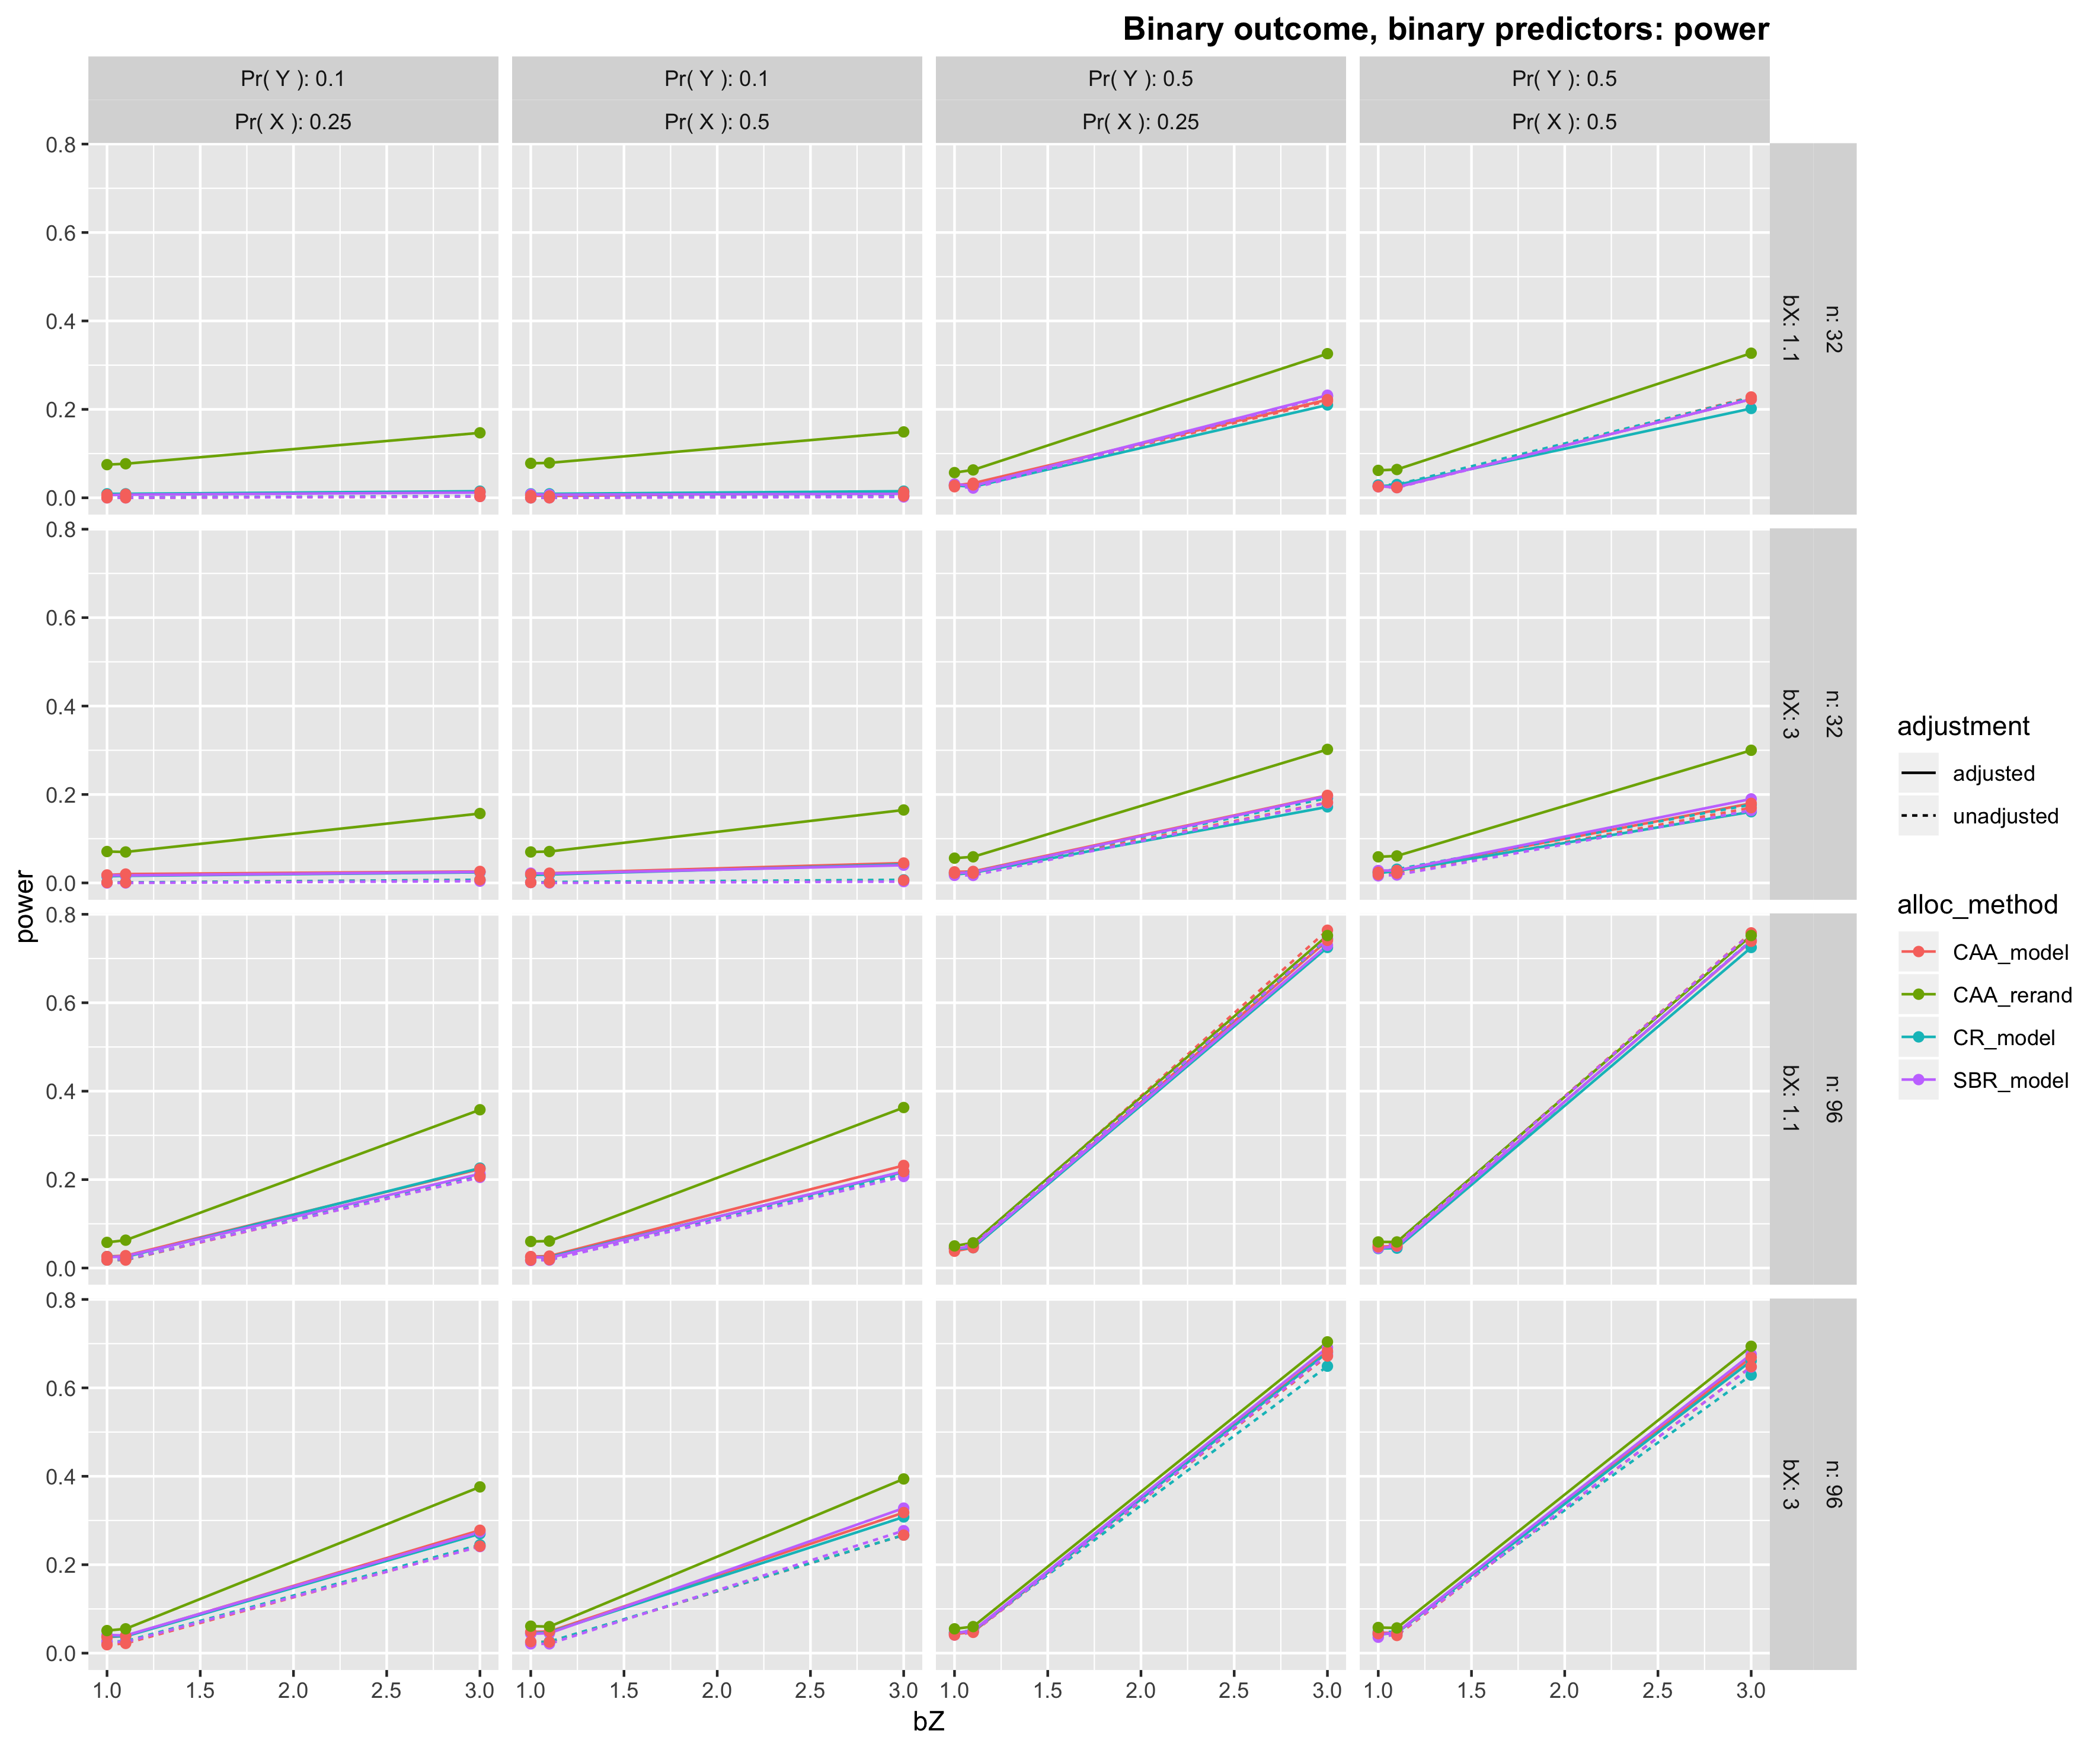
\includegraphics[width=\linewidth]{figures/b1_power_all_methods_adj_unadj}
	\caption{Batch 1: Power}
	\label{fig:b1p}
\end{figure}

\begin{figure}[H]
	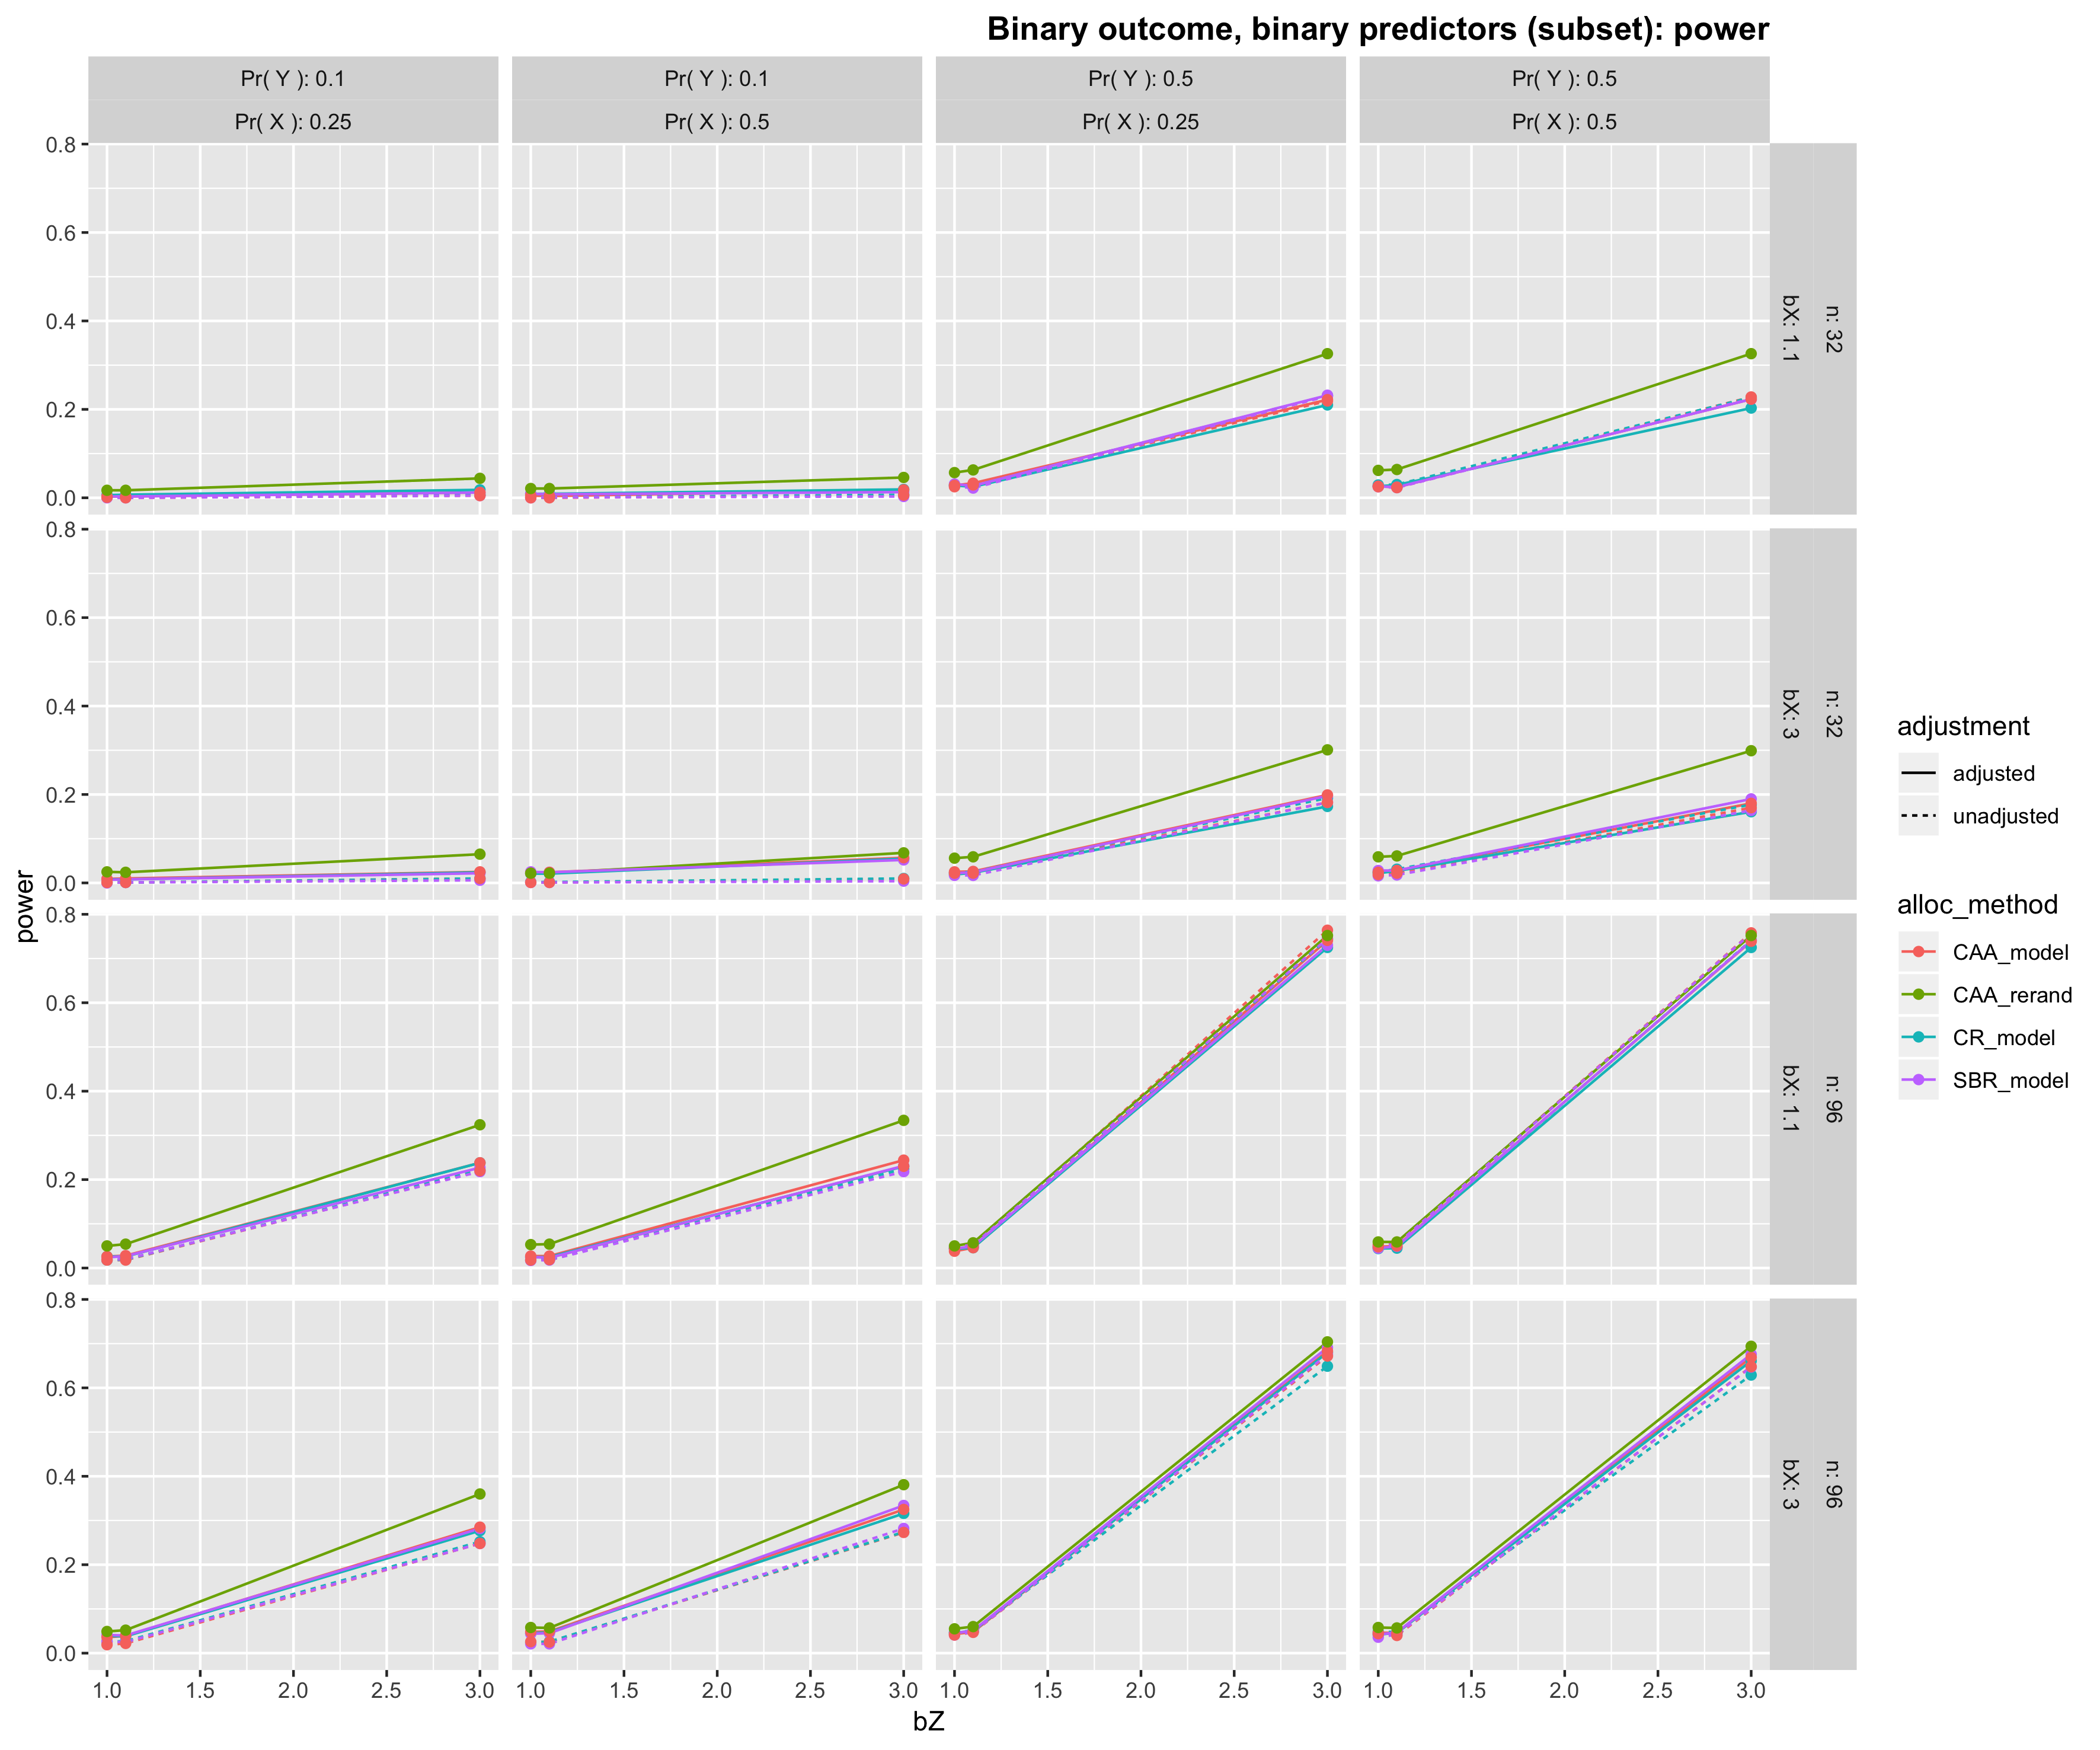
\includegraphics[width=\linewidth]{figures/b1_sub_power_all_methods_adj_unadj}
	\caption{Batch 1 subset: Power}
	\label{fig:b1sp}
\end{figure}

\begin{figure}[H]
	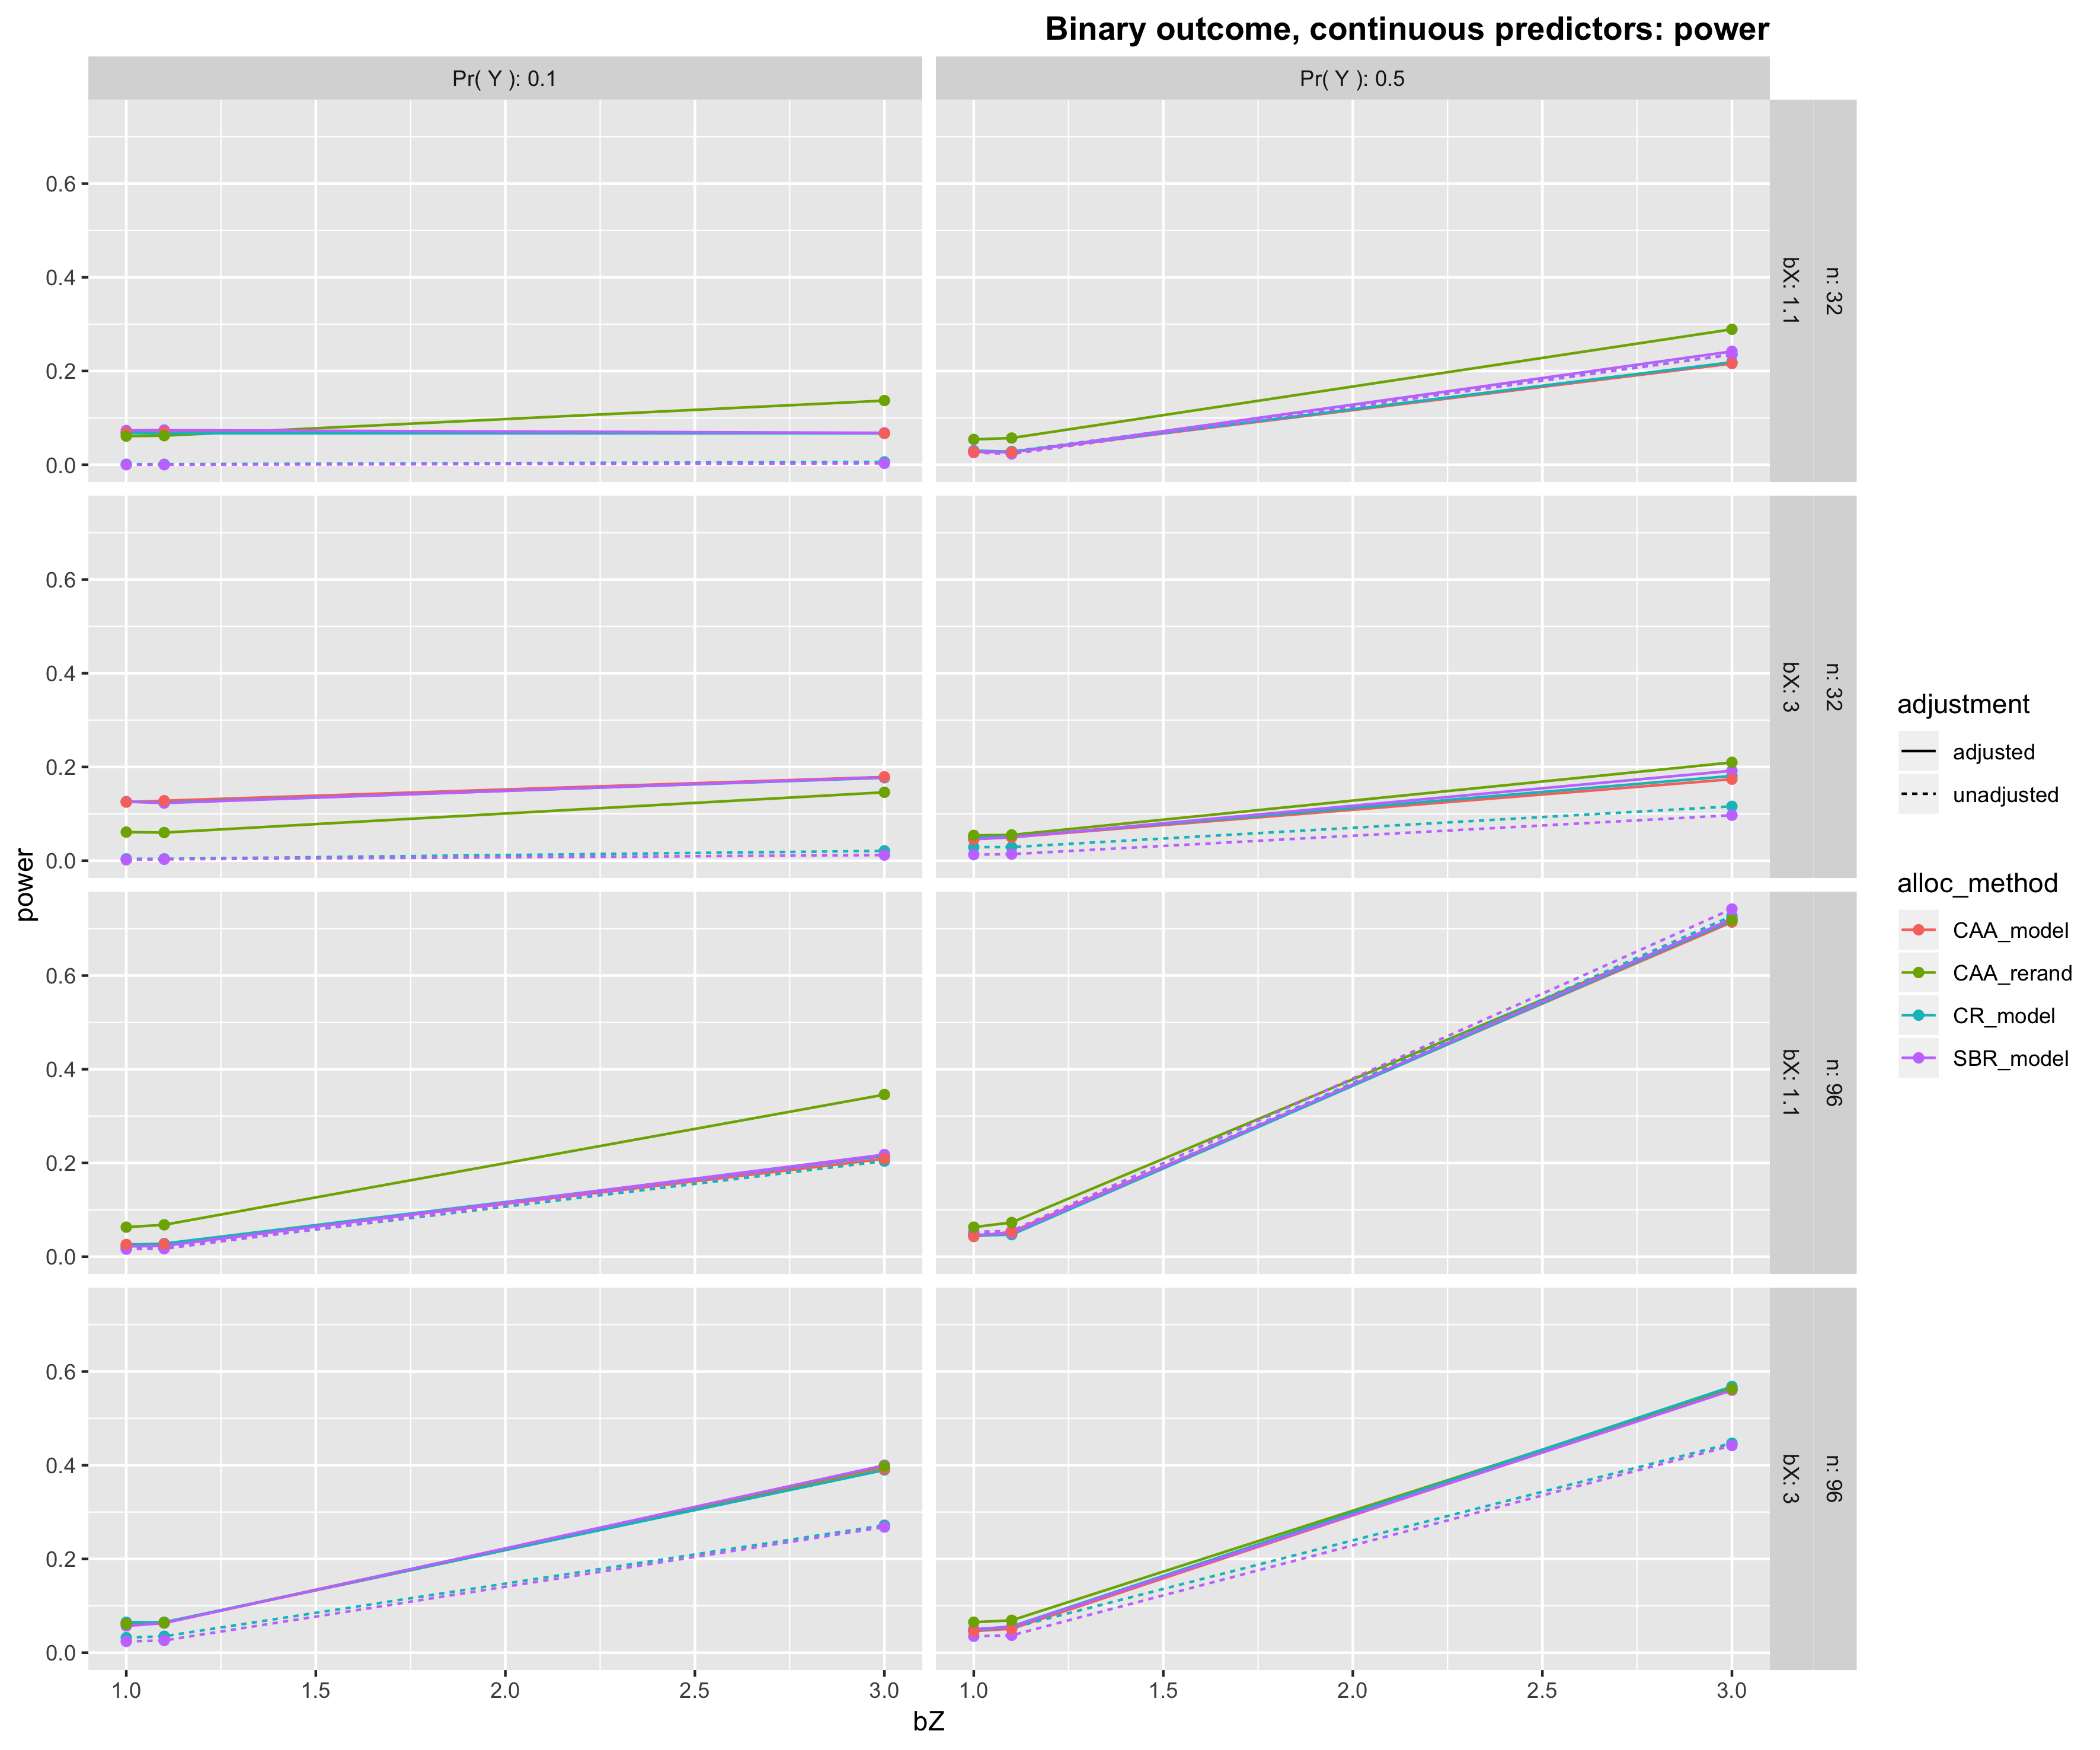
\includegraphics[width=\linewidth]{figures/b2_power_all_methods_adj_unadj}
	\caption{Batch 2: Power}
	\label{fig:b2p}
\end{figure}

\begin{figure}[H]
	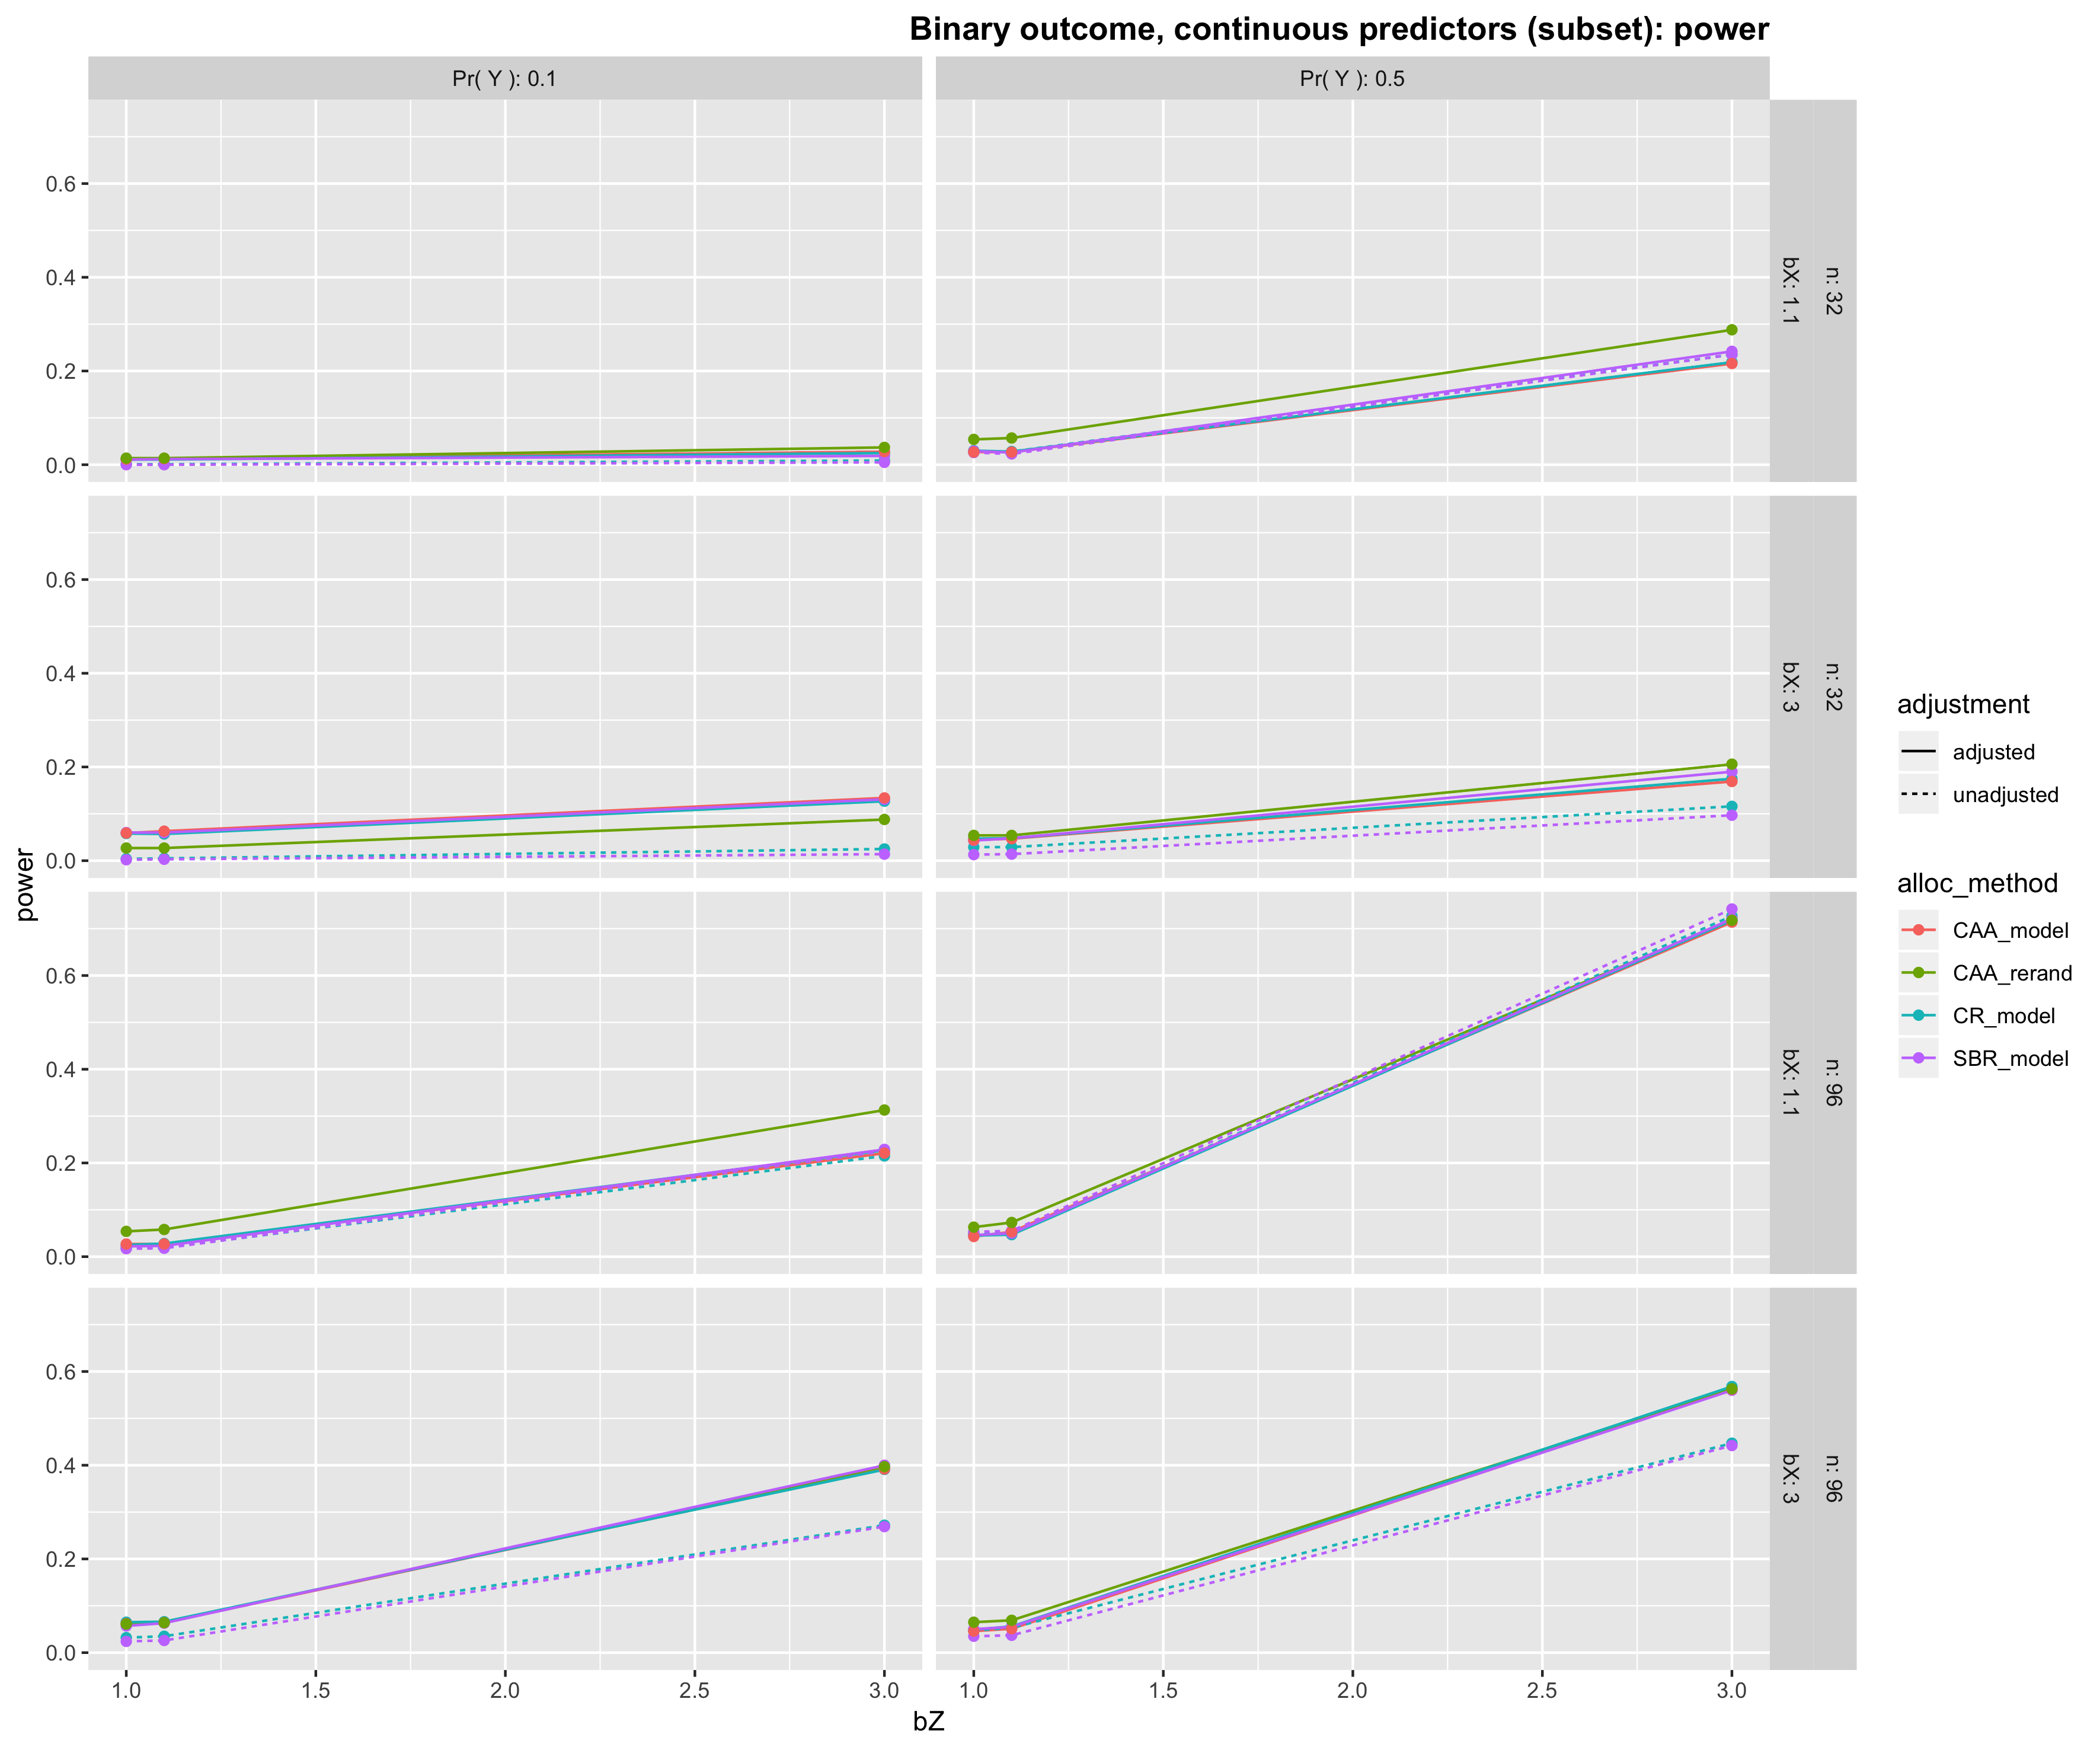
\includegraphics[width=\linewidth]{figures/b2_sub_power_all_methods_adj_unadj}
	\caption{Batch 2 subset: Power}
	\label{fig:b2sp}
\end{figure}

\begin{figure}[H]
	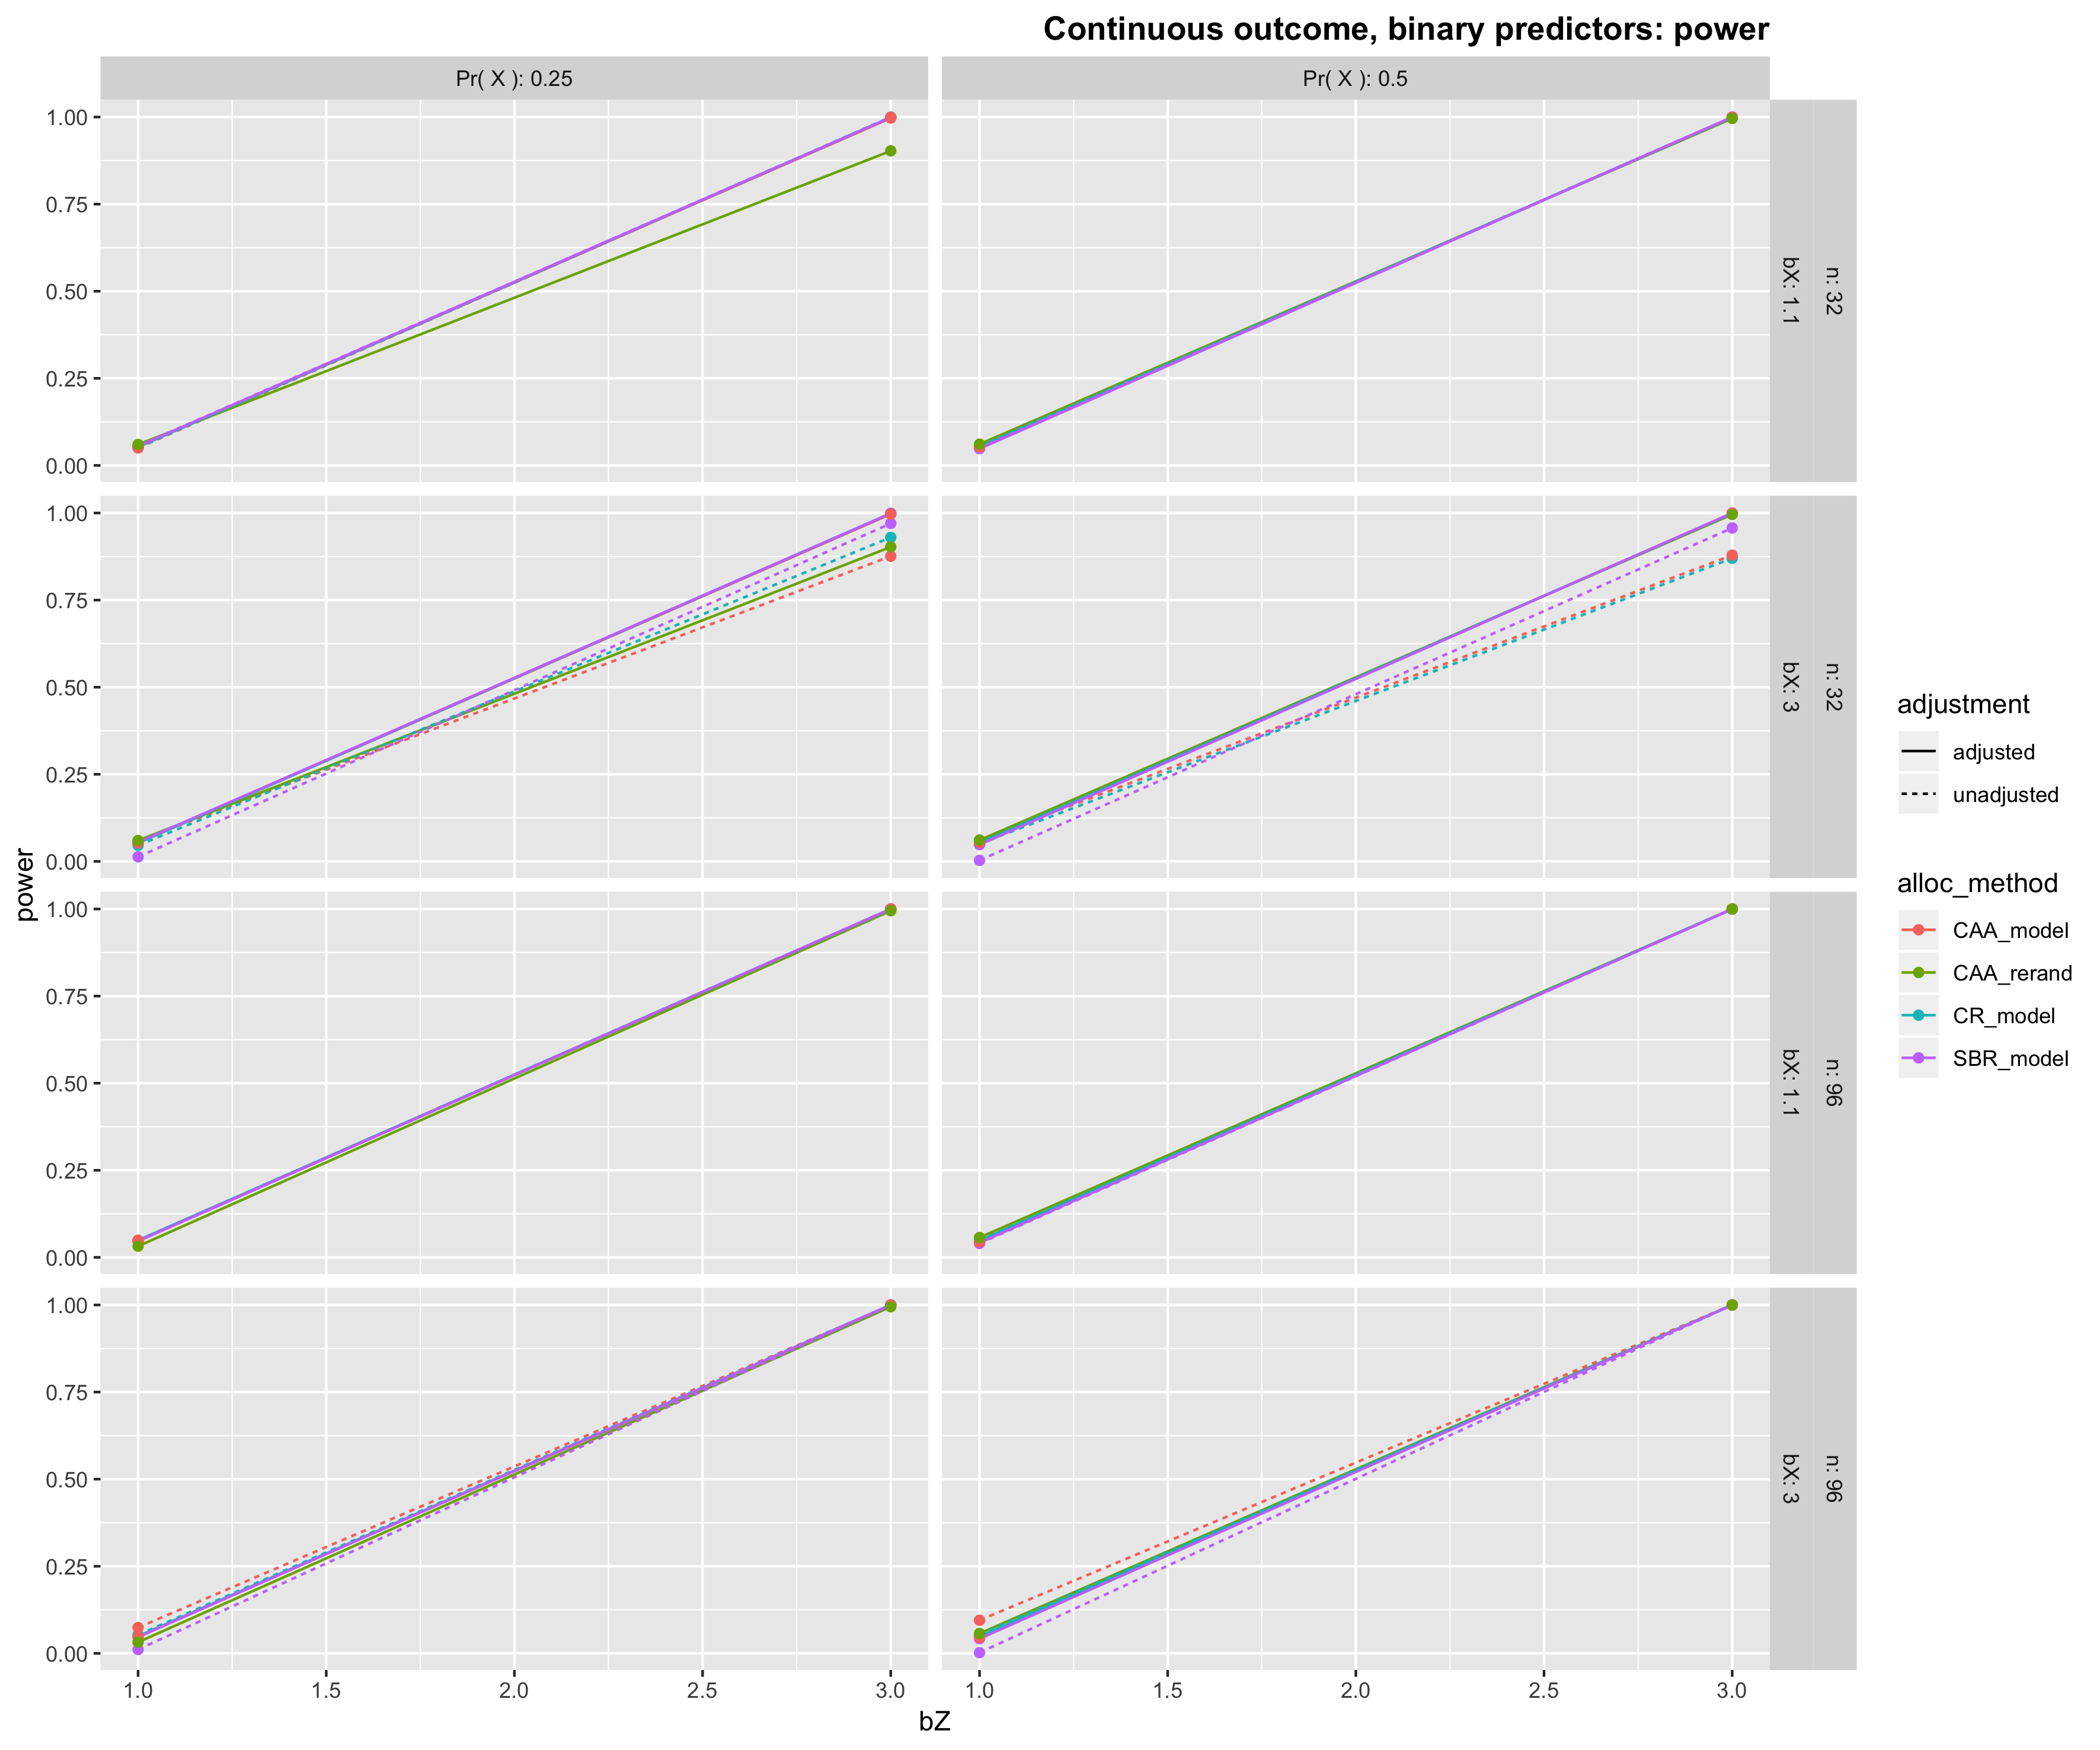
\includegraphics[width=\linewidth]{figures/b3_power_all_methods_adj_unadj}
	\caption{Batch 3: Power}
	\label{fig:b3p}
\end{figure}

\begin{figure}[H]
	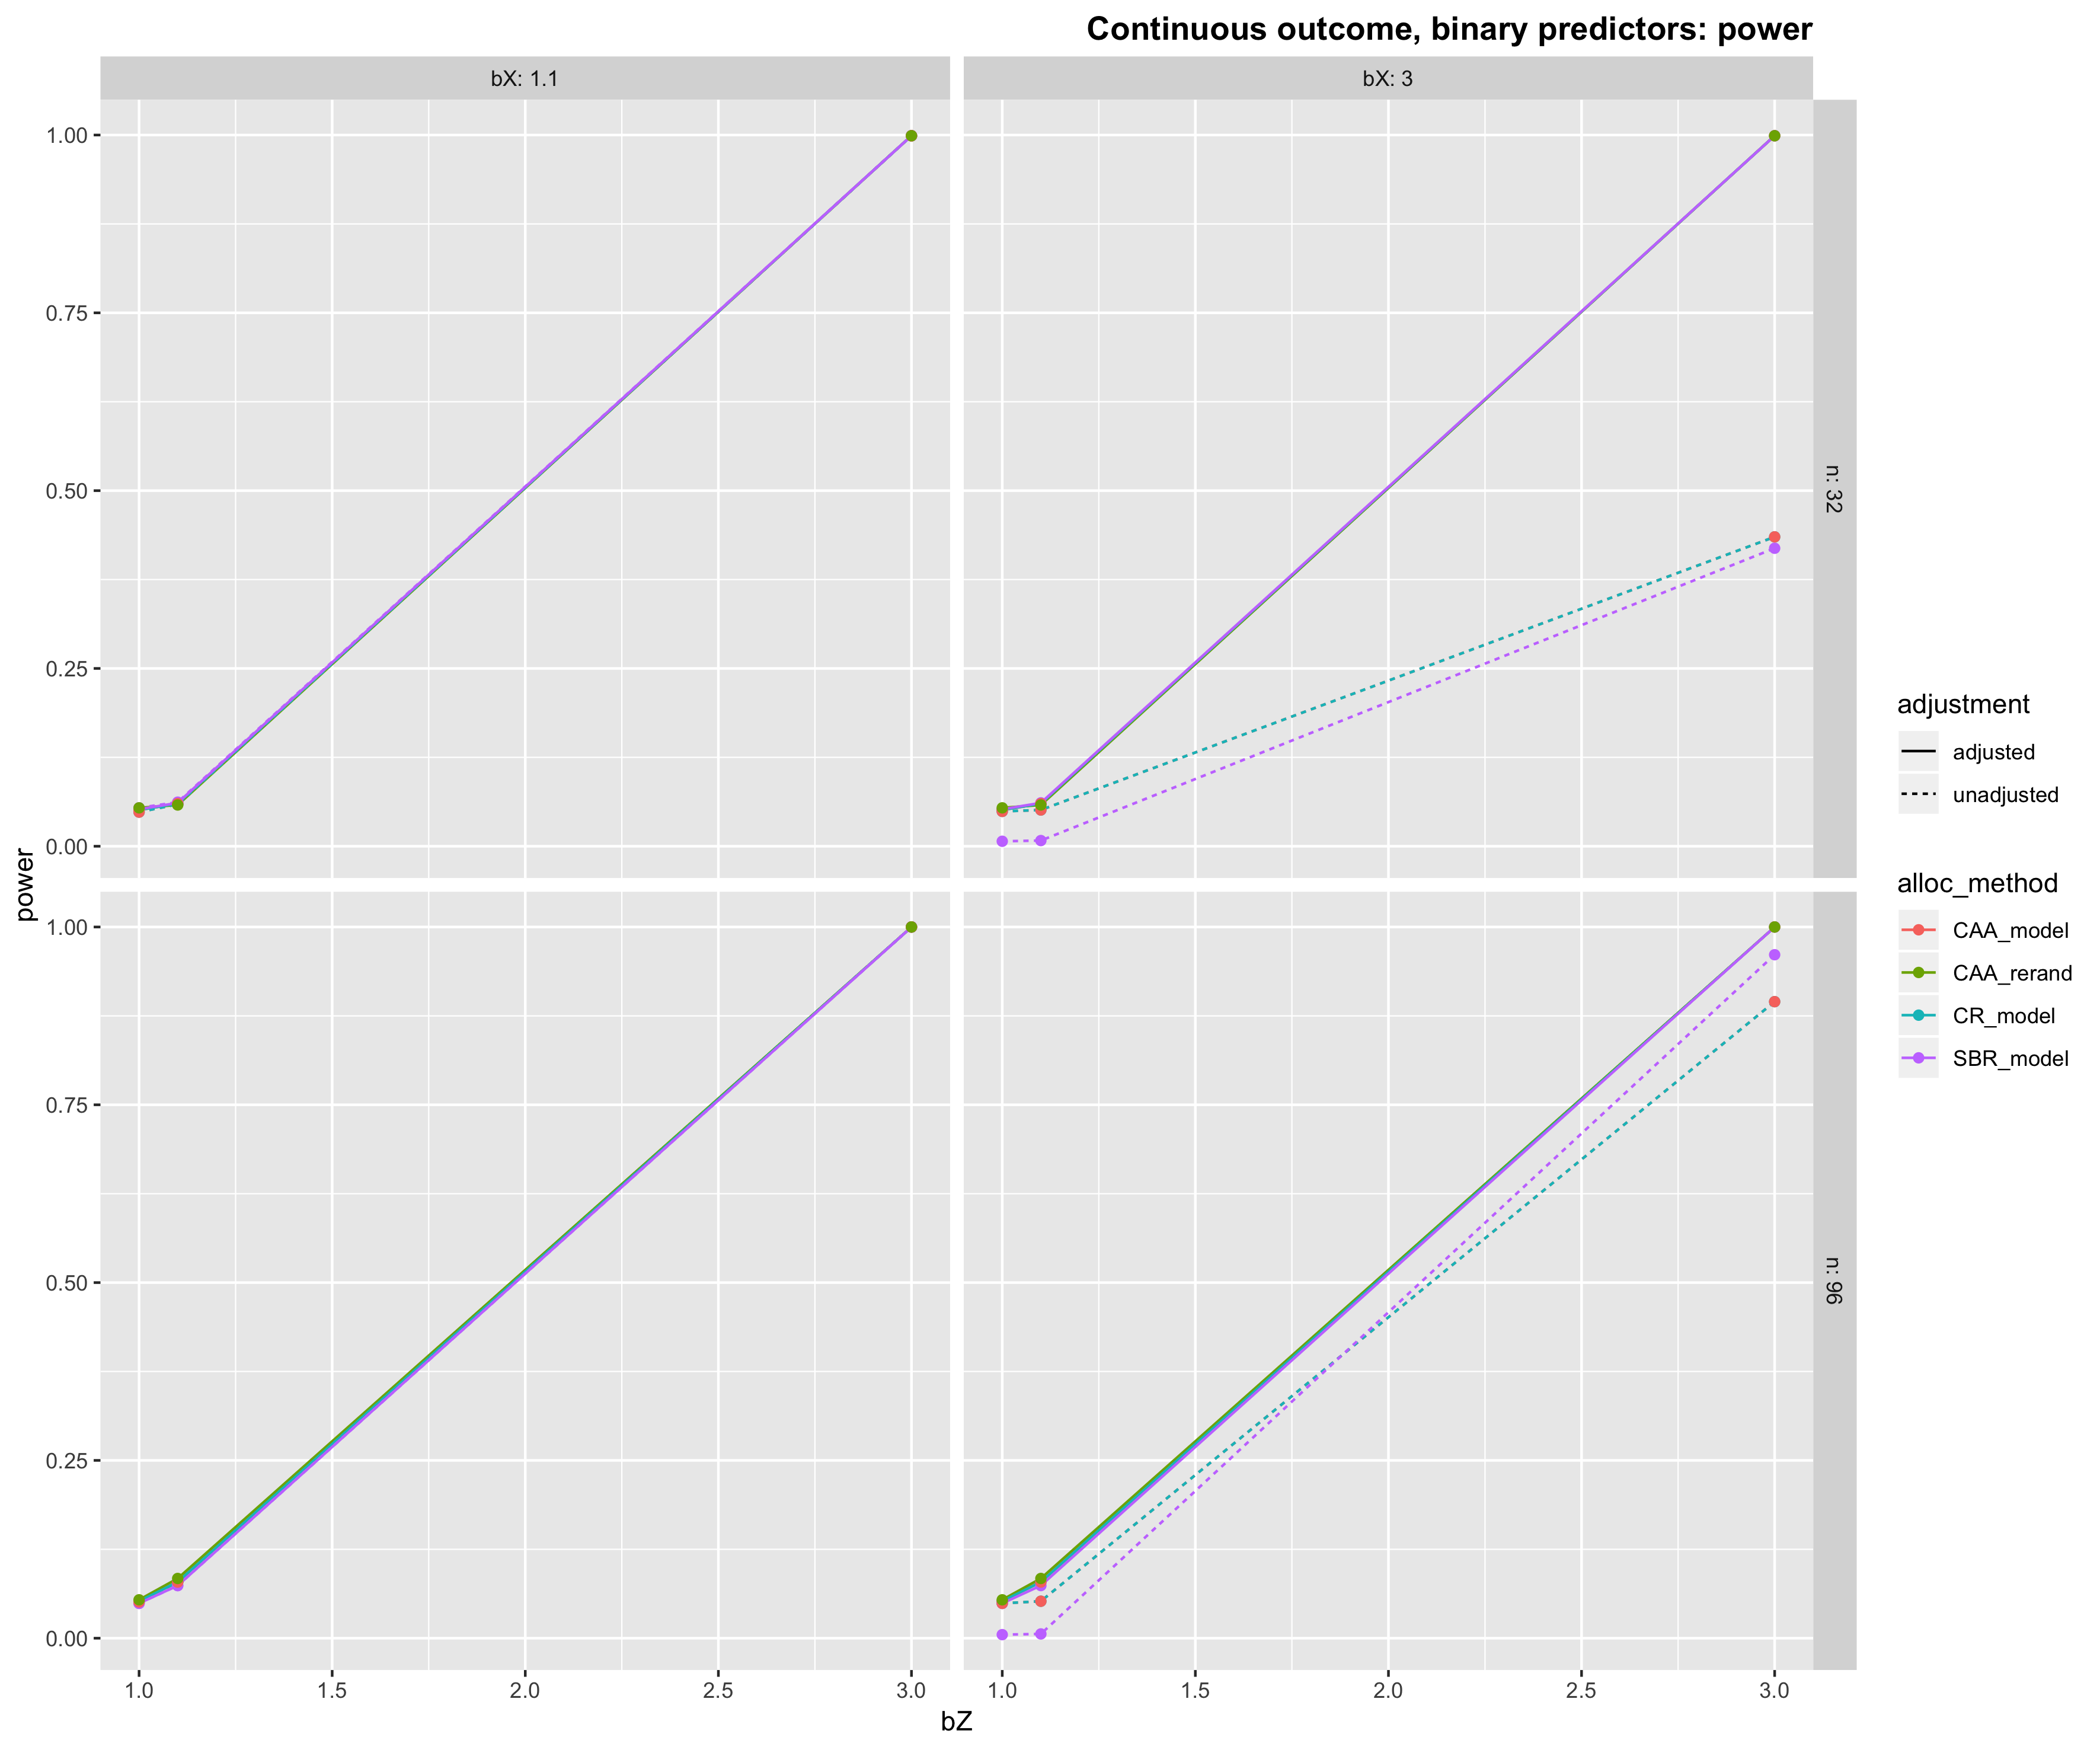
\includegraphics[width=\linewidth]{figures/b4_power_all_methods_adj_unadj}
	\caption{Batch 4: Power}
	\label{fig:b4p}
\end{figure}